%!TEX root = ../../main.tex

The rank of a Tucker decomposition, given by the size of $\mathcal{G}$, directly
impacts the amount of compression, so the choice of rank is consequential. If
the decomposition's ranks are large, then great accuracy is achieved at the cost
of poor compression. If the decomposition's ranks are small, then great
compression is achieved at the cost of poor accuracy. This is known as the
tensor decomposition trade-off as seen in
\Cref{fig:tensor_decomposition_trade_off}. It is applied to all forms of
decompositions, but it is specially relevant here. 

\begin{figure}[ht!]
    \centering
    \begin{tikzpicture}

    % Seesaw beam (tilted from -5 to 5)
    \draw[thick] (-5,-0.5) -- (5,0.5);
    
    % Fulcrum (yellow triangle)
    \fill[yellow] (0,0) -- (-0.5,-1) -- (0.5,-1) -- cycle;

    % Rotation angle to match the beam tilt
    \def\tiltangle{5.7} % positive to match the upward slope from left to right

    % Left box - Compression (rotated to match beam angle)
    \node[draw=blue!50, fill=blue!10, text width=2.8cm, minimum height=1cm,
          align=center, anchor=south west, rotate=\tiltangle] at (-4.8,-0.455) {\textbf{Compression}};
    
    % Right box - Accuracy (rotated to match beam angle)
    \node[draw=blue!50, fill=blue!10, text width=2.8cm, minimum height=1cm,
          align=center, anchor=south west, rotate=\tiltangle] at (1.7,0.2) {\textbf{Accuracy}};
    
    
\end{tikzpicture}
    \caption{The Tensor Decomposition Trade-Off}
    \label{fig:tensor_decomposition_trade_off}
\end{figure}

To know compression beforehand, we specify the size of the core tensor
$\mathcal{G}$. In the 3-way case, we specify the array of ranks $\mathbf{r} =
[q, r, s]$, or in the $d$-way case, $\mathbf{r} = [r_1, \hdots, r_d]$. Because
we know the ranks beforehand, this is called the \textbf{rank-specified}
formulation, and with it, we also know the compression ratio before hand as seen
in \Cref{eq:compression_ratio} for the 3-way case. In this formulation, we
cannot say in advance what the accuracy will be.

\begin{equation} \label{eq:compression_ratio}
    \frac{mnp}{qrs + qm + nr + sp} \approx \frac{mnp}{qrs}
\end{equation}

To know accuracy beforehand, we specify the maximum relative error threshold
$\epsilon$ of the tucker approximation. The 3-way case of the relative error can
be seen in \Cref{eq:rel_error}. This is called the \textbf{error-specified}
formulation, where we cannot say in advance what the compression will be. 

\begin{equation} \label{eq:rel_error}
    \frac{\| \mathcal{X} - \llbracket \mathcal{G}; \mathbf{U, V, W} \rrbracket \|}{\|\mathcal{X}\|} \leq \epsilon
\end{equation}

We now go on a journey to understand two of the main Tucker Decomposition
algorithms; STHOSVD and HOOI. STHOSVD is the more popular of the two for many
reasons, but one of them is that the algorithm works in both rank- and
error-specified formulation. HOOI, on the other hand, can only work in the
rank-specified formulation. 


\section{Tucker Algorithms} \label{sec:Tucker Algorithms}
    %!TEX root = ../../main.tex

Recall from \Cref{sec:Tucker Tensors and The Tucker Decomposition} that a Tucker
decomposition of a tensor $\mathcal{X}\in \mathbb{R}^{n_1\times \cdots \times
n_d}$ approximates $\mathcal{X}$ as a product of a core tensor $\mathcal{G} \in
\mathbb{R}^{r_1 \cdots r_d}$ and factor matrices $\mathbf{U}_j \in
\mathbb{R}^{n_k\times r_k} \forall k \in [d]$ where $\mathcal{X} \approx
\mathcal{\hat{X}} = \mathcal{G} \times_1 \mathbf{U}_1 \cdots \times
\mathbf{U}_d$. The optimal rank-$\mathbf{r}$ Tucker decomposition of
$\mathcal{X}$ can be expressed as a solution to the rank-specified optimization problem

\begin{equation}\label{eq:tuckeropt-rank}
    \begin{aligned}
        \min \quad & \| \mathcal{X} - (\mathcal{G} \times_1 \mathbf{U}_1 \cdots \times \mathbf{U}_d)\| \\ 
        \text{subject to } &\mathcal{G} \in \mathbb{R}^{r_1\times \cdots \times r_d}, \mathbf{U}_{k} \in \mathbb{R}^{n_k\times r_k} \forall k\in [d].
    \end{aligned}
\end{equation}

Alternatively, the error-specified formulation of the Tucker approximation
problem is given as

\begin{equation}\label{eq:tuckeropt-err}
    \begin{aligned}
        \min \quad & \prod_{j=1}^d r_j + \sum_{j=1}^d n_jr_j & \\ 
        \text{subject to } &\mathcal{G} \in \mathbf{R}^{r_1\times \cdots r_d}, \mathbf{U}_{j} \in \mathbb{R}^{n_k\times r_k} \forall k\in [d] \\
        \text{and}\quad  & \| \mathcal{X} - (\mathcal{G} \times_1 \mathbf{U}_1 \cdots \times \mathbf{U}_d) \| \leq \epsilon \|\mathcal{X}\|.
    \end{aligned}
\end{equation}

\subsection{STHOSVD} \label{sec:sthosvd} 

    We start with the state-of-the art algorithm that is capable of performing
    both rank-specified and error-specified formulations. \Cref{alg:STHOSVD}
    showcases the $d$-way construction of the STHOSVD algorithm. This method
    approximately solves either \cref{eq:tuckeropt-rank} or
    \cref{eq:tuckeropt-err} by unfolding the $k^\text{th}$ mode of the input
    tensor, computing its leaft leading singular vectors (LLSV), and then
    performing a TTM with the result to truncate the $k^\text{th}$ mode of rank
    $r_k$. Once all factor matrices have been computed, the truncated tensor has
    rank $\mathbf{r}$.

    A relative error error of $\epsilon$ can be achieved by selecting $r_k$ in
    the LLSV computation such that \(\sum_{i=r_k+1}^{n_k}\varSigma_i^2 \leq
    \epsilon^2 \|\mathcal{X}\|^2/d\), where $\varSigma_i$ is the $i^\text{th}$ largest
    singular value of the $j^\text{th}$ unfolding, see \cite{BK25} for more
    details. There are several algorithms one could choose in line
    \ref{line:sthosvd_llsv} to compute $\mathbf{U}_k$. We assume that such
    computation is performed via the eigenvalue decomposition (EVD) of the Gram
    matrix $\mathbf{G}_{(k)}\mathbf{G}_{(k)}$. 

    \begin{algorithm}
        \caption{STHOSVD}
        \label{alg:STHOSVD}
        \begin{algorithmic}
            \State{\textbf{Input:} Tensor $\mathcal{X} \in \mathbb{R}^{n_1 \times \cdots \times n_d}$} % \vspace{-0.75em}}
            \State{\hspace{3.25em} Ranks \textbf{R} $ = r_1, \dots, r_d$ \textbf{OR} relative error tolerance $\epsilon > 0$} % \vspace{-0.75em}}
            
            \State{\textbf{Output:} TTensor $\mathcal{T}$ of ranks \textbf{R} with $\mathcal{T \approx X}$ \textbf{OR} E{\footnotesize \text{RR}} $\equiv ||\mathcal{X - T}|| \leq \epsilon ||\mathcal{X}||$}
            \Function{STHOSVD}{$\mathcal{X}$, \textbf{R} or $\epsilon$}
                \State{\textbf{if} $\epsilon$ is defined \textbf{then} $\bar{\epsilon} \gets (\epsilon / \sqrt{d})\cdot||\mathcal{X}||$}
                \State{$\mathcal{G \gets X}$}
                \For{$k = 1, \dots, d$}
                    \State{$[U_k, \epsilon_k] \gets \textcolor{blue}{LLSV}(G_{(k)}, r_k \text{ or } \bar{\epsilon})$}\label{line:sthosvd_llsv} \Comment{$r_k$ leading left sing. vectors of residual} 
                    \State{$\mathcal{G} \gets \mathcal{G \times_k} U^\intercal_k$}\label{line:sthosvd_ttm} \Comment{compress in mode $k$}
                \EndFor{}
                \vspace{10pt}
                \State{E{\footnotesize \text{RR}} $\gets \displaystyle \sqrt{\sum_{k=1}^d \epsilon_k^2}$} \Comment{equivalent to $||\mathcal{X - T}||$}
                \vspace{10pt}
                \State{\textbf{return} [$\mathcal{G}, U_{1:d}$, E{\footnotesize \text{RR}}]} \Comment{$\mathcal{T \equiv \{G; \textit{$U_{1:d}$}\}}$}
            \EndFunction
        \end{algorithmic}
    \end{algorithm}

\subsection{Classic HOOI} \label{sec:Classic HOOI} 

    Our protagonist is given in \cref{alg:Classic-HOOI} and is an alternative
    method for solving the rank-specified formulation of the Tucker
    approximation problem
    \cite{kroonenberg1980principal,de2000best,kapteyn1986approach}. HOOI is a
    block coordinate descent method and so it requires initial factor matrices.
    Historically, the output factor matrices of STHOSVD have been used as input
    factor matrices for the HOOI algorithm, as the latter has often been as an
    aditional algorithm to just cheaply clean up the error. However, random
    factor matrices can be used and generally no more than two iterations are
    requireed to get a good approximation, often only one iteration is enough to
    get a descent one. 

    HOOI iteratively updates each factor matrix by performing a TTM with all but
    the $k^\text{th}$ factor matrix to obtain an intermediate tensor
    $\mathcal{Y}$ and computing the LLSV of $\mathbf{Y}_{(k)}$. The core tensor
    $\mathcal G$ can be computed oce, at the end, or at the end of every
    iteration in order to computate a per-iteration approximation error. 

    \begin{algorithm}
        \caption{HOOI}
        \label{alg:Classic-HOOI}
        \begin{algorithmic}
            \State{\textbf{Input:} Tensor $\mathcal{X} \in \mathbb{R}^{n_1 \times \cdots \times n_d}$}
            \State{\hspace{3.25em} Either Ranks \textbf{R} $ = r_1, \dots, r_d$}
            \State{\hspace{3.25em} Maximum Number of Iterations}
            
            \State{\textbf{Output:} TTensor $\mathcal{T}$ of ranks \textbf{R} with $\mathcal{T \approx X}$}
            \Function{HOOI}{$\mathcal{X}$, \textbf{R} or $\epsilon$}
                \State{Initialize factor matrices $U_{1:d}$ randomly}
                \State{$\mathcal{G \gets X}$}
                \For{Maximum Number of Iterations}
                    \For{$k = 1, \dots, d$}
                        \State{$\mathcal{Y = X} \times_1 U_1^\intercal \times_2 \cdots \times_{k-1} U_{k-1}^\intercal \times_{k+1} U_{k+1}^\intercal \times_{k+2} \cdots \times_d U_d^\intercal$}
                        \State{$U_k \gets \text{LLSV}(Y_{(k)}, r_k)$}
                    \EndFor{}
                \EndFor{}
                \State{$\mathcal{G \gets Y} \times_d U_d^\intercal$} \Comment{update core}
                \State{\textbf{return} [$\mathcal{G}, U_{1:d}$]} \Comment{$\mathcal{T \equiv \{G; \textit{$U_{1:d}$}\}}$}
            \EndFunction
        \end{algorithmic}
    \end{algorithm}

    HOOI is a good algorithm, but it can be better. As previously mentioned, we
    introduce three optimizations for the HOOI algorithm in an attempt to make
    it more competitive against STHOSVD. 

\subsection{Motivating HOOI Optimizations}

\subsection{HOOI's Dimension Trees Optimization}
    Adapting ranks in each HOOI iteration is a low order cost, however, the cost
    of TTMs is a factor of $d$ more expensive than in STHOSVD. We can reduce the
    cost of TTMs by avoiding redundant computations. Notice that for $k = 1$ in
    \cref{alg:Classic-HOOI} the following multi-TTM is computed $\mathcal{Y} =
    \mathcal{X} \times_2 \mathbf{U}_{2}^\intercal \times_3
    \mathbf{U}_{3}^\intercal \cdots \times_d \mathbf{U}_{d}$. At $k = 2$ the
    multi-TTM is $\mathcal{Y} = \mathcal{X} \times_2 \mathbf{U}_{1}\times
    \times_3 \mathbf{U}_{3}^\intercal \cdots \times_d \mathbf{U}_{d}$. By
    comparing the two multi-TTMs we can see that $d - 2$ TTMs are the same
    (namely 3 to $d$). So we can reuse results from one multi-TTM to the next by
    memoizing intermediate results. This idea, organized using so-called
    ``dimension trees'', was first used in the context of CP decompositions
    \cite{PTC13a} and has been applied to Tucker computations as well
    \cite{kaya2019computing,MLB24}. \Cref{fig:dimtree} shows an example
    dimension tree as we implement them for an order-$6$ tensor where each node
    represents the set of modes in which a TTM has not been performed. At the
    root of the tree, no TTMs have been performed, so the tensor is $\mathcal{X}$.
    Each notch in an edge of the tree represents a TTM in the labeled mode. At
    each leaf node, TTMs in all modes but one have been performed, so we update
    the factor matrix in that mode by performing LLSV. The core tensor $\mathcal{G}$
    is updated at the last leaf node by perform a TTM between the (memoized)
    intermediate tensor and the factor matrix corresponding to the last leaf
    node.

    \begin{figure}
        \centering
        %!TEX root = ../main.tex

\begin{tikzpicture}[scale=2]

    \node (123456) at (4,2) {$\{1,2,3,4,5,6\}$};
    \node (123) at (2,1) {$\{1,2,3\}$};
    \node (1) at (1,0) {$\{1\}$};
    \node (23) at (3,0) {$\{2,3\}$};
    \node (2) at (2,-1) {$\{2\}$};
    \node (3) at (4,-1) {$\{3\}$};

    \node (456) at (6,1) {$\{4,5,6\}$};
    \node (4) at (5,0) {$\{4\}$};
    \node (56) at (7,0) {$\{5,6\}$};
    \node (5) at (6,-1) {$\{5\}$};
    \node (6) at (8,-1) {$\{6\}$};
    
    \draw (123456) -- (123)
    	node[pos=0.25, circle, fill=black, inner sep=1pt,label=above left:{\tiny 6}] {}
	node[pos=0.5, circle, fill=black, inner sep=1pt,label=above left:{\tiny 5}] {}
	node[pos=0.75, circle, fill=black, inner sep=1pt,label=above left:{\tiny 4}] {};
    \draw (123456) -- (456)
    	node[pos=0.25, circle, fill=black, inner sep=1pt,label=above right:{\tiny 1}] {}
	node[pos=0.5, circle, fill=black, inner sep=1pt,label=above right:{\tiny 2}] {}
	node[pos=0.75, circle, fill=black, inner sep=1pt,label=above right:{\tiny 3}] {};
    \draw (123) -- (1)
	node[pos=0.33, circle, fill=black, inner sep=1pt,label=above left:{\tiny 3}] {}
	node[pos=0.66, circle, fill=black, inner sep=1pt,label=above left:{\tiny 2}] {};
    \draw (123) -- (23)
	node[pos=0.5, circle, fill=black, inner sep=1pt,label=above right:{\tiny 1}] {};
    \draw (456) -- (4)
	node[pos=0.33, circle, fill=black, inner sep=1pt,label=above left:{\tiny 6}] {}
	node[pos=0.66, circle, fill=black, inner sep=1pt,label=above left:{\tiny 5}] {};
    \draw (456) -- (56)
	node[pos=0.5, circle, fill=black, inner sep=1pt,label=above right:{\tiny 4}] {};
    \draw (23) -- (2)
	node[pos=0.5, circle, fill=black, inner sep=1pt,label=above left:{\tiny 3}] {};
    \draw (23) -- (3)
	node[pos=0.5, circle, fill=black, inner sep=1pt,label=above right:{\tiny 2}] {};
    \draw (56) -- (5)
	node[pos=0.5, circle, fill=black, inner sep=1pt,label=above left:{\tiny 6}] {};
    \draw (56) -- (6)
	node[pos=0.5, circle, fill=black, inner sep=1pt,label=above right:{\tiny 5}] {};
    

    \end{tikzpicture}
    

        \label{fig:dimtree}
        \caption[A 6-way Dimension Tree]{Illustration of multi-TTM memoization
        for an order-$6$ tensor. Each node in the tree shows the set of modes in
        which multiplication has not been performed. Each notch in an edge is a
        TTM in the labeled mode.  Factor matrices are computed at each leaf node
        in the mode shown. $\mathcal{G}$ is updated in the last leaf node.}
    \end{figure}

    \Cref{alg:dimtree} shows the HOOI iteration using dimension tree memoization
    implemented recursively.


    \begin{algorithm}
        \caption{Recursive HOOI iteration via dimension trees}
        \label{alg:dimtree}
        \begin{algorithmic}[1]
            \Function{[$\mathcal{G},\{\mathbf{U}_{k}\}] = $HOOI-DT}{$\mathcal{X},\{\mathbf{U}_{k}\},\mathbf{m},\mathbf{r}$}
                \If{length($\mathbf{m}) = 1$}
                    \State $\mathbf{U}_{m} = $ \Call{LLSV}{$\mathbf{X}_{(m)}, \mathbf{U}_m, r_m$}
                    \If{$m=d$}
                        \State $\mathcal{G} = \mathcal{X} \times_d \mathbf{U}_{m}^\intercal$
                    \EndIf
                \Else
                    \State Partition $\mathbf{m} = [\mathbf{\mu},\mathbf{\eta}]$ \State $\mathcal{X} = \mathcal{X} \scaleobj{1.7}{\times}_{k \in \mathbf{\mu}} \mathbf{U}_{k}^\intercal$
                    %$\mathcal{X} = \mathcal{X} \times_{\mathbf{\mu}(1)} \mathbf{U}__{\mathbf{\mu}(1)}^\top \times \dots \times_{\mathbf{\mu}(end)} \mathbf{U}__{\mathbf{\mu}(end)}^\top$
                    \State $[\mathcal{G},\{\mathbf{U}_{k}\}] = \Call{HOSI-DT}{\mathcal{X},\{\mathbf{U}_{k}\},\mathbf{\eta}, \mathbf{r}$}
                    \State $\mathcal{X} = \mathcal{X} \scaleobj{1.7}{\times}_{k \in \mathbf{\eta}} \mathbf{U}_{k}^\intercal$
                    %$\mathcal{X} = \mathcal{X} \times_{\mathbf{\eta}(1)} \mathbf{U}__{\mathbf{\eta}(1)}^\top \times \dots \times_{\mathbf{\eta}(end)} \mathbf{U}__{\mathbf{\eta}(end)}^\top$
                    \State $[\mathcal{G},\{\mathbf{U}_{k}\}] =\Call{HOSI-DT}{\mathcal{X},\{\mathbf{U}_{k}\}, \mathbf{\mu},\mathbf{r}$}
                \EndIf
            \EndFunction
        \end{algorithmic}
    \end{algorithm}

\subsection{HOOI's Subspace Iteration Optimization} \label{sec:HOOI's Subspace Iteration Optimization}

    So far, we have assumed that the LLSVs of a matrix $\mathbf{A}$ are obtained
    as the eigenvectors of the Gram matrix, $\mathbf{A}\mathbf{A}^\intercal$.
    % which can be seen in \cref{alg:gram_llsv}
    The next algorithmic improvement we introduce is to compute the leading left
    singular vectors by using subspace iterations. \Cref{alg:subiter} shows a
    single subspace iteration, but in principle, the computations could be
    repeated to improve accuracy.

    \begin{algorithm}
        \caption{LLSV via Subspace Iteration}
        \label{alg:subiter}
        \begin{algorithmic}[1]
        \Function{$\mathbf{Q} = $ \textcolor{red}{LLSV}}{$\mathbf{A}, \mathbf{U}, r$}
    %        \If{$method == Gram+Eig$}
    %            \State $\Mx{Z} = \Tm{B}{j} \Tm{B}{j}'$
    %            % \Comment{Comm: all-to-all and reduce-scatter}
    %            \State $\sqr{\Mx{Q}{j}, \Mx{\Lambda}} = \Call{eig}{\Mx{Z}}$
    %        \ElsIf{$method == Sub.~Iter.$}
    %	   \State $\mathbf{U}_ = \mathbf{U}_(:, 1:r)$
                \State $\mathbf{G} = \mathbf{U}^\intercal \mathbf{A} $ \label{line:SI-TTM}
                % \Comment{Comm: reduce-scatter}
                \State $\mathbf{Z} = \mathbf{A} \mathbf{G}^\intercal$ \label{line:SI-contract}
                % \Comment{Comm: reduce + broadcast}
                \State $[\mathbf{Q}, \sim, \sim] = \Call{QRCP}{\mathbf{Z}}$ \label{line:SI-QRCP}
    %        \EndIf
    %        \State $\Mx{Q}{j} = \Mx{Q}{j}(:, 1:r_j)$
        \EndFunction
        \end{algorithmic}
        %\AD{Not sure if I like branching based on $method$}
        %\GB{I think I will change this to LLSV-SI and make variables more generic}
    \end{algorithm}

    We note that the input matrix $\mathbf{A}$ is $\mathbf{Y}_{(k)}$ from
    \cref{alg:Classic-HOOI} or $\mathbf{X}_{(m)}$ from \cref{alg:dimtree},
    which is the result of an all-but-one multi-TTM, and the input matrix
    $\mathbf{U}$ is the factor matrix from the previous HOOI iteration. This implies
    that the temporary matrix $\mathbf{G}$ in \cref{alg:subiter} is an unfolding of
    the core tensor corresponding to the current set of factor matrices. That
    is, the matrix multiplication in line \ref{line:SI-TTM} is a TTM, which we
    implement using existing TuckerMPI subroutines. The multiplication in
    line \ref{line:SI-contract} is a tensor contraction in all modes but one between
    the core tensor and the result of an all-but-one multi-TTM, which is not
    implemented in TuckerMPI. Our parallel algorithm mimics the computation of
    the Gram matrix of a tensor unfolding, but it is a nonsymmetric operation
    and has different costs. Finally, we perform QR with column pivoting in
    line \ref{line:SI-QRCP} to orthonormalize the subspace iteration result and also
    order the columns to aid in core analysis, which is discussed in
    \cref{sec:HOOI's Adaptive Rank Optimization}. We choose to do only a single subspace iteration
    because we use an accurate initialization (from the previous HOOI iteration)
    and because high accuracy of a HOOI subiteration is less of a priority than
    high accuracy of the full HOOI iteration.

\subsection{HOOI's Adaptive Rank Optimization} \label{sec:HOOI's Adaptive Rank Optimization}

    \begin{figure}
        \centering
        \begin{tikzpicture}[scale=1,namenode/.style={scale=1}]
    % These distances can be meddled with to get you what you want
    % Within reason...
    \def\ix{2.5} %
    \def\iy{2.5} %
    \def\iz{1.75} %
    \def\corescale{1.75} % Has to be more than 1
    \def\rot{90}
    \def\r{0.25}
    \def\rx{\ix/\corescale}
    \def\ry{\iy/\corescale}
    \def\rz{\iz/\corescale}
    \def\redux{0.15}
    \def\reduy{0.15}
    \def\reduz{0.35}
    
    % Give figure's starting point and draw a rectange
    \coordinate (TFrontLowerLeft) at (0,0);
    \draw (TFrontLowerLeft) rectangle ++ (\ix,\iy);
 
    % This scope draws the top face of the cube
    \begin{scope}[shift={(TFrontLowerLeft)}, canvas is zx plane at y=\iy,rotate=\rot]
       \draw (0,0) rectangle ++ (\ix,\iz);
    \end{scope}
 
    % This scope draws the left side of the cube
    \begin{scope}[shift={(TFrontLowerLeft)},canvas is zy plane at x=\ix,rotate=90]
       \draw (0,0) rectangle ++ (\iy,\iz); %
    \end{scope}
 
    % This writes the tensor name in the front face of the cube
    \node[namenode] at ($(TFrontLowerLeft) + (0.5*\ix, 0.5*\iy)$)  {$\mathbf{\mathcal{T}}$};
 
    % This writes the equal sign to the side of the cube
    \coordinate (ApproxCtr) at ($(TFrontLowerLeft) + (0.75+\ix+0.4*\iz,0.7*\iy)$);
    \node[namenode] at (ApproxCtr) {$\approx$};
 
    % First Factor Matrix
    \coordinate (AFrontLowerLeft) at ($(ApproxCtr) + (0.75,-\ry)$);
    \draw (AFrontLowerLeft) rectangle ++ (\rx,\iy);
    \node[namenode] at ($(AFrontLowerLeft) + (0.5*\rx, 0.5*\iy)$)  {$A$};
    \draw[red, fill=red, fill opacity = 0.5] (AFrontLowerLeft) rectangle ++ (\rx-\redux,\iy);
 
    % This scope draws the top face of the cube
    \coordinate (CFrontLowerLeft) at ($(AFrontLowerLeft) + (0.5 + \rx, 0.25*\ix)$);
    \draw (CFrontLowerLeft) rectangle ++ (\rx,\ry);
    \coordinate (SubCore) at ($(CFrontLowerLeft) + (0, \reduy)$);
    \draw[red, fill=red, fill opacity = 0.5] (SubCore) rectangle ++ (\rx - \redux, \ry - \reduy);
 
    \begin{scope}[shift={(CFrontLowerLeft)}, canvas is zx plane at y=\ry,rotate=\rot]
       \draw (0,0) rectangle ++ (\rx,\rz);
    \end{scope}
    \begin{scope}[shift={(SubCore)}, canvas is zx plane at y=\ry-\reduy,rotate=\rot]
       \draw[red, fill=red, fill opacity = 0.5] (0,0) rectangle ++ (\rx-\redux,\rz-\reduz);
    \end{scope}
    
    % This scope draws the left side of the cube
    \begin{scope}[shift={(CFrontLowerLeft)},canvas is zy plane at x=\rx,rotate=90]
       \draw (0,0) rectangle ++ (\ry,\rz); %
    \end{scope}
    \begin{scope}[shift={(SubCore)},canvas is zy plane at x=\rx-\redux,rotate=90]
       \draw[red, fill=red, fill opacity = 0.5] (0,0) rectangle ++ (\ry-\reduy,\rz-\reduz); %
    \end{scope}
 
    % This writes the core name in the front face of the cube
    \node[namenode] at ($(CFrontLowerLeft) + (0.5*\rx, 0.5*\ry)$)  {$\mathbf{\mathcal{G}}$};
 
    % Second Factor Matrix
    \coordinate (BFrontLowerLeft) at ($(CFrontLowerLeft) + (\rx + 0.75*\rz, 0.15*\rz)$);
    \draw (BFrontLowerLeft) rectangle ++ (\ix,\ry);
    \node[namenode] at ($(BFrontLowerLeft) + (0.5*\ix, 0.5*\ry)$)  {$B$};
    \draw[red, fill=red, fill opacity = 0.5] ($(BFrontLowerLeft) + (0, \reduy)$) rectangle ++ (\ix,\ry-\reduy);
 
    % Third Factor Matrix
    \begin{scope}[shift={($(CFrontLowerLeft) + (0.25*\rz,-0.25*\rz)$)},canvas is zx plane at y=\iy,rotate=90]
       \draw (0,\r) rectangle ++ (\rz*1.3,\iz*1.15);
    \end{scope}
    \begin{scope}[shift={($(CFrontLowerLeft) + (0.25*\rz,-0.25*\rz)$)},canvas is zx plane at y=\iy,rotate=90]
       \draw[red, fill=red, fill opacity = 0.5] (0,\r) rectangle ++ (\rz*1.3 - \reduz,\iz*1.15);
    \end{scope}
    \node[namenode] at ($(CFrontLowerLeft) + (1*\rx,2.75*\rz)$) {$C$};
 
         
 \end{tikzpicture}
        \caption{Adaptive HOOI}
        \label{fig:adaptive_hooi}
    \end{figure}

    A significant disadvantage of HOOI is that it solves only the rank-specified
    formulation of the Tucker approximation problem, whereas STHOSVD can
    adaptively select ranks based on a relative error tolerance. We propose a
    technique that allows HOOI to automatically adapt ranks to meet a
    user-specified relative error tolerance. 

    Recall that for the error-specified formulation, given an error tolerance
    $\varepsilon$ and an initial rank estimate $\mathbf{r}$, our method adaptively
    finds a Tucker decomposition $\mathbf{\hat{X}} = [\mathcal{G}; \mathbf{U}_{1}, \dots,
    \mathbf{U}_{d}]$ for a tensor $\mathcal{X} \in \mathbb{R}^{n_1 \times \dots \times
    n_d}$ such that $\| \mathbf{\hat{X}} - \mathcal{X} \| \leq \varepsilon \| \mathcal{X} \|$.
    We start with a typical HOOI iteration using our initial rank estimate
    $\mathbf{r}$, partially compressing our tensor in all modes except mode $j$ and
    updating factor matrix $\mathbf{U}_{j}$ to be the first $r_j$ left singular
    vectors of the partially compressed tensor. Once all modes have been
    processed in this manner, we check the error of the approximation at that
    point. 
    Whereas in clasical HOOI the core is only updated after the iterations, here
    we compute the core tensor at the end of everu iteration and perform error
    analysis on it. To check the error, we use the identity that for orthonormal
    matrices $\mathbf{U}_{1},\dots,\mathbf{U}_{d}$ and $\mathcal{G} = \mathcal{X} \times_1
    \mathbf{U}_{1}\intercal \times \dots \times_d \mathbf{U}_{d}^\intercal$, the approximation error can be
    written as $\| \mathcal{X} - \mathbf{\hat{X}} \|^2 = \| \mathcal{X} - \mathcal{G} \times_1
    \mathbf{U}_{1} \times \dots \times_d \mathbf{U}_{d} \|^2 = \| \mathcal{X} \|^2 - \| \mathcal{G}
    \|^2$ (\cite[Proposition 6.3]{BK25}). If the current Tucker approximation is
    not sufficiently accurate, we increase all ranks by a factor $\alpha$ and
    perform the next HOOI iteration. If the current approximation satisfies the
    error threshold, then we can optimize over all rank truncations by analyzing
    the core tensor's entries.
    We can thus estimate the relative error in the approximation by computing
    $\| \mathcal{G} \|$, and choosing the next rank $\mathbf{r}$ so that $\|
    \mathcal{G}(\mathbf{1}:\mathbf{r})\|^2 \approx (1 - \varepsilon^2) \| \mathcal{X} \|^2.$ 
    Specifically, we solve the optimization problem
    \begin{equation}\label{eq:rankcond}
    \begin{aligned}
    \min_{\mathbf{r}}  \quad & \Pi_{j=1}^d r_j + \Sigma_{j=1}^{d} n_j r_j,\\ 
    \text{ subject to } &\|\mathcal{G}(\mathbf{1}:\mathbf{r}) \|^2 \geq (1 - \varepsilon^2) \| \mathcal{X} \|^2.
    \end{aligned}
    \end{equation}
    This computes the leading subtensor of $\mathcal{G}$ that minimizes the size of
    the Tucker approximation and also satisfies the error threshold. Note that
    any subtensor of the core, along with the corresponding columns of the
    factor matrices, is a valid Tucker approximation with error determined by
    the norm of the core subtensor. The optimal subtensor need not be a leading
    one, but we order factor matrix columns to concentrate the weight of
    $\mathcal{G}$ towards the entry of smallest index value so that the heuristic of
    searching over only leading subtensors is reasonable.

    If such a rank $\mathbf{r}$ exists, we set our next rank as the closest
    index satisfying \eqref{eq:rankcond} and truncate to that rank before
    iterating. If no $\mathbf{r}$ exists, our current rank is too small, so we
    increase it by a small factor $\alpha$ before trying again. Typically,
    $\alpha \approx 2$ is sufficient. The details of this algorithm, are
    described in \ref{alg:Adaptive-HOOI}. In practice, we do the optimization
    problem above in a way that minimizes the memory footprint. We do so by
    exploiting HOOI's form of the immediate core $\mathcal{G}$. We use the
    immediate form to compute its cumulative sum of the squared core
    $\mathcal{G}^2$ (square all entries in the core) and then consider all
    values of this cumulative sum squared tensor to find the first instance that
    satisfies the error tolerance to get the new ranks.

    \begin{algorithm}
        \caption{Adaptive HOOI}
        \label{alg:Adaptive-HOOI}
        \begin{algorithmic}
            \Function{performCoreAnalysis}{$\mathcal{G}, \epsilon, \mathbf{r}$}
                \If{$||\mathcal{G} ||^2 \geq (1 - \epsilon^2)||\mathcal{X}||^2$}
                    \State{Find \textbf{r} = arg min $||\mathcal{G}(1:\textbf{r}) ||^2$}
                    \State{$\hspace{0.1375\linewidth}$subject to $||\mathcal{G}(1:\textbf{r}) ||^2 \geq (1 - \epsilon^2)||\mathcal{X}||^2$}
                    \State{}
                    \State{Truncate $\mathcal{G}, A, B, C$ according to $\mathbf{r}$}
                \Else{}
                    \State{\textbf{r} = $\alpha$ \textbf{r}}
                    \State{Increase columns of $ A, B, C$ according to $\mathbf{r}$}
                \EndIf{}
                \State{\textbf{return} $\mathbf{r}$}
            \EndFunction{}
        \end{algorithmic}
    \end{algorithm}

    % \begin{eqnarray*}
    %     \text{min} ||\mathcal{X - G} \times U_1 \times_2 \cdots \times_d U_d || \\
    %     \text{subject to } \mathcal{G} \in \mathbb{R}^{n_1 \times \cdots \times n_d}, U_k \in \mathbb{R}^{n_k \times r_k} \text{ } \forall k \in [d]
    % \end{eqnarray*}
    
    % Now suppose we have a relative error tolerance of how accurate we want
    % our approximation to be. Then the approximation must satisfy:
    % \begin{eqnarray*}
    %     \frac{||\mathcal{X - T}||}{||\mathcal{X}||} \leq \epsilon \\
    %     \frac{||\mathcal{X - T}||^2}{||\mathcal{X}||^2} \leq \epsilon^2 \\
    %     \therefore ||\mathcal{X - T}||^2 \leq \epsilon^2 \cdot ||\mathcal{X}||^2 \\
    %     \therefore ||\mathcal{X}||^2 - ||\mathcal{G}||^2 \leq \epsilon^2 \cdot ||\mathcal{X}||^2 \\
    %     \therefore ||\mathcal{X}||^2 - \epsilon^2 \cdot ||\mathcal{X}||^2 \leq ||\mathcal{G}||^2 \\
    %     \therefore (1 - \epsilon^2) \cdot ||\mathcal{X}||^2 \leq ||\mathcal{G}|| \\
    % \end{eqnarray*}
    
    % We can thus estimate the relative error in the approximation by
    % computing $||\mathcal{G}||^2$ and choosing the next rank-\textbf{R} so
    % that $||\mathcal{G}(1:\textbf{R}) ||^2 \approx (1 -
    % \epsilon^2)||\mathcal{X}||^2$. Specifically, we solve the optimization
    % problem
    % \begin{eqnarray*}
    %     \underbrace{\text{arg min}}_\textbf{R} ||\mathcal{G}(1:\textbf{R})||^2 \\
    %     \text{subject to } ||\mathcal{G}(1:\textbf{R}) ||^2 \geq (1 - \epsilon^2)||\mathcal{X}||^2
    % \end{eqnarray*}
    
    
    % \begin{algorithm}
    %     \caption{Adaptive HOOI}
    %     \label{alg:Adaptive-HOOI}
    %     \begin{algorithmic}
    %         \State{\textbf{Input:} Tensor $\mathcal{X} \in \mathbb{R}^{n_1 \times \cdots \times n_d}$}
    %         \State{\hspace{3.25em} Either Ranks \textbf{R} $ = r_1, \dots, r_d$}
    %         \State{\hspace{3.25em} Maximum Number of Iterations}
    %         \State{\hspace{3.25em} Rank Size Increase Rate $\alpha$}
            
    %         \State{\textbf{Output:} TTensor $\mathcal{T}$ of ranks \textbf{R} with $\mathcal{T \approx X}$}
    %         \Function{AdaptiveHOOI}{$\mathcal{X}$, \textbf{R} or $\epsilon$}
    %             \State{Initialize factor matrices $U_{1:d}$ randomly}
    %             \State{$\mathcal{G \gets X}$}
    %             \For{Maximum Number of Iterations}
    %                 \For{$k = 1, \dots, d$}
    %                     \State{$\mathcal{Y = X} \times_1 U_1^\intercal \times_2 \cdots \times_{k-1} U_{k-1}^\intercal \times_{k+1} U_{k+1}^\intercal \times_{k+2} \cdots \times_d U_d^\intercal$}
    %                     \State{$U_k \gets \text{LLSV}(Y_{(k)}, r_k)$}
    %                 \EndFor{}
    %                 \State{$\mathcal{G \gets Y} \times_d U_d^\intercal$} \Comment{update core}
    %                 \If{$||\mathcal{G} ||^2 \geq (1 - \epsilon^2)||\mathcal{X}||^2$}
    %                     \State{Find \textbf{R} = arg min $||\mathcal{G}(1:\textbf{R}) ||^2$,subject to $||\mathcal{G}(1:\textbf{R}) ||^2 \geq (1 - \epsilon^2)||\mathcal{X}||^2$}
    %                     \State{$\mathcal{G = G}(1:\textbf{R}, U_k = U_k(1:r_k) \text{  } \forall k \in [d]$}
    %                 \Else{}
    %                     \State{\textbf{R} = $\alpha$ \textbf{R}}
    %                 \EndIf{}
    %             \EndFor{}
    %             \State{\textbf{return} [$\mathcal{G}, U_{1:d}$]} \Comment{$\mathcal{T \equiv \{G; \textit{$U_{1:d}$}\}}$}
    %         \EndFunction
    %     \end{algorithmic}
    % \end{algorithm}
    

\section{The TuckerMPI Library}
    %!TEX root = ../../main.tex

\begin{center}
    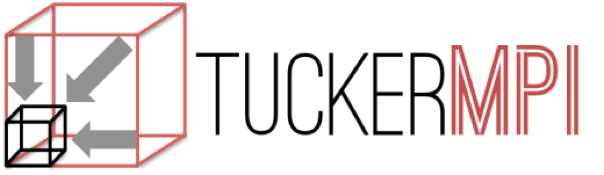
\includegraphics[scale=0.5]{tikz/chapter3/TuckerMPI-logo.png}
\end{center}

TuckerMPI uses $P$ processors organized into a $d$-dimensional $P_1\times \cdots
\times P_d$ grid such that $P = \prod_{i=1}^{d} P_i$ and that each processor
stores a $1/P$ fraction of $\mathcal{X}$. Our analysis will assume $\mathcal{X}
\in \mathbb{R}^{n\times \cdots \times n}$ and $\mathcal{G} \in
\mathbb{R}^{r\times \cdots \times r}$ to simplify cost comparison across
algorithms.

\subsection{TuckerMPI's STHOSVD} \label{sec:TuckerMPI's STHOSVD}
    \subsubsection{STHOSVD's Computational Complexity} \label{STHOSVD's Computational Complexity}

        The cost of LLSV in line \ref{line:sthosvd_llsv} is given by
        \begin{equation*}
            \sum_{j=1}^{d} \left(\frac{r^{j-1}n^{d-j+2}}{P} + \mathcal{O}(n^3)\right) \approx \frac{n^{d+1}}{P} + \mathcal{O}(dn^3),
        \end{equation*}
        where the first term is the cost of computing the $n \times n$ Gram matrix and
        the second term is the cost of sequentially computing the EVDs to leading order.
        %We perform the Eigendecomposition sequentially on a single processor and communicate $\Mx{U}_j$.
        After $\mathbf{U}_{k}$ is computed, $\mathcal{Y}$ is truncated by
        performing the TTM in line \ref{line:sthosvd_ttm}, which costs
        \begin{equation*}
            2\sum_{j=1}^{d} \frac{r^j n^{d-j+1}}{P} \approx 2\frac{rn^d}{P}.
        \end{equation*}
        Computing the Gram matrix is a factor of $\nicefrac{n}{2r}$ more expensive than
        the TTM and is the dominant cost for $n \gg r$. Sequentially truncating $\mathcal{Y}$
        leads to decreasing dimensions, so the algorithm is typically dominated by the
        first Gram matrix computation. Note that the EVD is not parallelized, which can
        be a barrier to parallel scaling when a single tensor dimension is large. We
        summarize the leading order STHOSVD flops cost in \cref{tab:flops} (shown in
        red).

    \subsubsection{STHOSVD's Communication Complexity} \label{sec:STHOSVD's Communication Complexity}

        TuckerMPI's parallel algorithm for LLSV explicitly forms the Gram
        matrix, $\mathbf{G} = \mathbf{Y}_{(k)}\mathbf{Y}_{(k)}^\intercal$,
        where $\mathbf{Y}_{(k)}$ is redistributed (if necessary) to a 1D column
        layout across $P$ processors, and then sequentially computes the EVD of
        $\mathbf{G}$. After redistribution of $\mathbf{G}$, each processor
        computes a local Gram matrix which can be sum-reduced (or all-reduced)
        prior to the EVD. At iteration $k$, the number of entries in
        $\mathcal{Y}$ is $r^{j-1}n^{d-j+1}$. The Gram matrix that is computed in
        each mode is of size $n \times n$, so the total communication cost is
        $dn^2$ for the all-reduce. Thus, the communication cost is given by
        \begin{equation*}
            \sum_{j=1}^{d} \bigg(\frac{r^{j-1}n^{d-j+1}}{P}\cdot \frac{P_j - 1}{P_j} + \mathcal{O}(n^2)\bigg) \approx \frac{n^{d}}{P}\cdot \frac{P_1 - 1}{P_1} + dn^2,
        \end{equation*}
        where we assume the redistribution cost is dominated by the first mode. However,
        note that there is no redistribution cost in mode $j$ if $P_j=1$. Finally, the
        parallel TTM also requires communication to perform a sum-reduce of local TTM
        results. Since the output of the TTM is largest in the first mode (of size
        $rn^{d-1}/P$), the communication cost of TTMs to leading order cost is
        \begin{equation*}
            \sum_{j=1}^{d} \frac{r^{j}n^{d-j}}{P}(P_j - 1) \approx \frac{rn^{d-1}}{P}(P_1 - 1).
        \end{equation*}
        Again, note there is no communication cost in mode $j$ if $P_j=1$.
        Because the largest data communicated occurs in mode 1, processor grids
        with $P_1=1$ are typically the fastest for STHOSVD (as we observe in our
        experiments). We summarize the STHOSVD communication costs in
        \cref{tab:comm} (shown in red).

\subsection{TuckerMPI's HOOI} \label{sec:TuckerMPI's HOOI}
    \subsubsection{HOOI's Computational Complexity} \label{sec:HOOI's Computational Complexity}

        Since HOOI is an iterative algorithm for Tucker decomposition, we analyze the
        cost of one HOOI iteration. Each HOOI iteration requires $d$ multi-TTMs, in all
        modes but mode-$j$, and $d$ LLSV computations to update factors matrices, in all
        modes. Once the factor matrices have been updated, the core tensor $\mathcal{G}$ is
        obtained by performing a TTM with the last factor matrix $\mathbf{U}{d}$. The cost
        of computing $d$ multi-TTMs is given by

        \begin{equation*}
            2d \sum_{i=1}^{d} \frac{r^i n^{d-i+1}}{P} \approx 2d\frac{rn^d}{P}.
        \end{equation*}

        The cost of each TTM decreases, so the first term in the summation (i.e. the
        first TTM) dominates. Multiplying the cost of the first TTM by $d$ yields the
        cost of $d$ multi-TTMs (i.e. one HOOI iteration). The cost of computing LLSV is
        given by
        \begin{equation*}
            d\frac{r^{d-1}n^2}{P} + \mathcal{O}(dn^3),
        \end{equation*}
        where the first term is the cost of computing the Gram matrix
        $\mathbf{Y}_{(k)}\mathbf{Y}_{(k)}'$ and the second term is the cost of
        computing the EVD. Finally, the core tensor at the end of each HOOI
        iteration is obtained by performing a TTM in mode-$d$ with the
        intermediate tensor $\mathcal{Y}$ and $\mathbf{U}_{d}$, which has a cost of
        $2\nicefrac{nr^{d}}{P}$ and is a lower order term. We summarize the
        leading order cost per HOOI iteration as implemented by TuckerMPI in
        \cref{tab:flops} (shown in red).


    \subsubsection{HOOI's Communication Complexity} \label{sec:HOOI's Communication Complexity}
        The communication cost of each iteration of HOOI is dominated by multi-TTMs and
        LLSV computations. Each TTM in the multi-TTM requires communication to perform a
        sum reduction to form $\mathcal{Y}$. Communication is required along the processor
        dimension corresponding to the mode in which a TTM is performed.
        %We consider two collectives for the sum reduction: a single reduce-scatter or $P_i$ reduces each with a different root.
        %If sufficient temporary storage is available, then a reduce-scatter is preferred as it is a factor of $2$ cheaper in bandwidth than performing $P_i$ reduces.
        %We assume that sufficient temporary storage is available and that the reduce-scatter is used.
        The size of $\mathcal{Y}$ decreases with each TTM, so the communication cost of a
        multi-TTM is dominated by the first TTM. Each HOOI iteration performs $d$
        multi-TTMs, where one iteration updates the factor matrix in the first mode.
        %We assume that the multi-TTM corresponding to $j=1$ in \Cref{alg:hooi} is performed in reverse order (starting with the mode-$d$ TTM) so that the largest TTM can be performed using a single GEMM call.
        The cost of communication for the multi-TTMs is given by
        \begin{multline*}
            \sum_{j=1}^d \bigg(\sum_{i=1}^{j-1} \frac{r^in^{d-i+2}}{P}(P_i-1) + \sum_{i=j+1}^{d} \frac{r^{i-1}n^{d-1+1}}{P}(P_i-1)\bigg) \\ \approx (d-1)\frac{rn^{d-1}}{P}(P_1 - 1) + \frac{rn^{d-1}}{P}(P_2 - 1).
        \end{multline*}
        The first term corresponds to the $d-1$ TTMs performed in the 1st mode and the
        second term corresponds to TTMs performed in the 2nd mode (for the multi-TTM in
        all but the 1st mode).
        %Each mode-$1$ TTM computes a local tensor of size $\frac{rn^{d-1}}{\Pi_{i = 2}^d P_i}$ which is reduce-scattered between processors in the $P_1$ dimension which yields a bandwidth cost of $\frac{rn^{d-1}}{P} (P_1 - 1)$ per TTM in the first mode.
        %When updating the first mode factor matrix, we perform the mode-$d$ TTM first.
        %The mode-$d$ TTM stores a local tensor of size $\frac{rn^{d-1}}{\Pi_{i = 1}^{d-1} P_i}$ which is communicated in the $P_d$ dimension.
        %Multiplying the cost of reduce-scatter in the mode-$1$ TTMs by $d-1$ and adding the cost of the mode-$d$ TTM (when $j = 1$) yields the total communication cost of multi-TTMs to leading order.

        Communication is also required when computing the LLSV in each mode.
        Using the same LLSV algorithm as in STHOSVD, the Gram matrix is computed
        in parallel followed by a sequential EVD. Computing the Gram matrix
        requires an all-to-all to redistribute $\mathbf{Y}_{(k)}$ so that it is
        stored in 1D-column layout. After redistribution
        $\mathbf{Y}_{k}\mathbf{Y}_{k}^\intercal$ is computed in parallel by
        performing local matrix-matrix multiplications that are sum-reduced to
        obtain the Gram matrix. The cost of communication for the LLSV is given
        by
        \begin{equation*}
            \frac{r^{d-1}n}{P} \sum_{i = 1}^{d}\left(\frac{P_i-1}{P_i}\right) + dn^2,
        \end{equation*}
        where the first term is the cost of all-to-all communication and the second term
        is the cost of sum reduction of the Gram matrix for one HOOI iteration (i.e. $d$
        calls to LLSV).
        %Each all-to-all requires redistribution of $\frac{nr^{d-1}}{P}$ local data which must be sent to $P_i$ processors, where $i$ is the mode in which LLSV is being computed.
        %This requires sending $P_i - 1$ messages each of size $\frac{1}{P_i} \cdot \frac{nr^{d-1}}{P}$.
        %Summing this cost over all $d$ modes yields the first term.
        %The second term is the cost of sum-reducing the $n$-dimensional Gram matrix, which has a message size cost of $n^2$ per mode.
        %Multiplying this cost by $d$ gives the second term.
        We summarize the HOOI communication costs as implemented by TuckerMPI in \Cref{tab:comm} (shown in red).


\subsection{TuckerMPI's Dimension Tree} \label{sec:TuckerMPI's Dimension Tree}
    \subsubsection{Dimension Tree Computational Complexity} \label{sec:Dimension Tree Computational Complexity}

        The flops cost of performing multi-TTMs using dimension trees is given by
        \begin{equation*}
            4 \sum_{i=1}^{d/2} \frac{r^i n^{d-i+1}}{P} + \mathcal{O} \left(d \sum_{i = d/2 + 1}^{d} r^i n^{d - i + 1}\right) \approx 4\frac{rn^d}{P},
        \end{equation*}
        where the first term is the cost of computing the TTMs in the first two branches
        (left and right of the root) in the dimension tree and the second term is the
        cost of computing the TTMs in all remaining branches. The largest TTMs in the
        first two branches dominate, so the cost of multi-TTMs is $4\cdot \nicefrac{rn^d}{P}$
        (i.e. the first TTM in each branch), which is a factor of $\nicefrac d2$ improvement over
        computing multi-TTMs directly. This cost is summarized in \Cref{tab:flops}.
    
    \subsubsection{Dimension Tree Communication Complexity} \label{sec:Dimension Tree Communication Complexity}

        Since the first TTM in each of the two multi-TTMs off the root dominate,
        the communication cost of multi-TTMs is given by
        \begin{equation*}
            \sum_{i=1}^{d/2}  \frac{r^in^{d-i-1}}{P}\left(P_i - 1 + P_{d-i+1} - 1\right) \approx   \frac{rn^{d-1}}{P} \left(P_1 + P_d - 2\right).
        \end{equation*}
        
        When traversing the right branch in the dimension tree shown in
        \cref{fig:dimtree}, TTMs are performed in the first $\nicefrac d2$ modes
        starting with mode $1$. The communication cost associated with TTMs in
        the right branch is the cost of a reduce-scatter on local data of size
        $\nicefrac{rn^{d-1}}{P}\cdot(P_1-1)$, which yields the first term. The
        second term is due to the communication cost associated with traversing
        the left branch in \cref{fig:dimtree}. TTMs in the left branch are
        performed in the last $\nicefrac d2$ modes starting with mode $d$. We
        perform left branch TTMs in reverse order because the mode $d$ TTM
        achieves higher local TTM performance due to the layout of the local
        tensor in memory. The communication cost associated with TTMs in the
        left branch is the same as the first term, except that the
        reduce-scatter is performed in the $P_d$ processor grid dimension.
        Therefore, processor grids with $P_1 = P_d = 1$ are typically the
        fastest for HOOI algorithms employing the dimension tree optimization
        (as we observe in our experiments).

        As shown in \cref{tab:flops,tab:comm}, introducing dimension trees
        memoization reduces the flops cost of TTMs in HOOI by a factor of $d/2$
        and the communication cost by a factor of $d-1$ in the first term.


\subsection{TuckerMPI's Subspace Iterations} \label{TuckerMPI's Subspace Iterations}
    \subsubsection{Subspace Iteration Computational Complexity.}
        Each subspace iteration requires two matrix-matrix multiplications and
        one QR decomposition. The first matrix-multiplication corresponds to the
        TTM $\mathcal{G}=\mathcal{Y} \times_k \mathbf{U}_{(k)}^\intercal$ (in the
        notation of \cref{alg:Classic-HOOI}) and the second computes the tensor
        contraction $\mathbf{Y}_{(k)}\mathbf{G}_{(k)}^\intercal$. The total computational cost of
        performing the TTM and contraction in each HOOI iteration is
        $4d\cdot\nicefrac{nr^d}{P}$. The cost of the QR decomposition of the
        matrix $\mathbf{Z} \in \mathbb{R}^{n\times r}$ in each HOOI iteration is
        $\mathcal{O}(dnr^2)$, where we assume a sequential QR decomposition. The
        total cost of performing subspace iteration in each mode across an
        entire HOOI iteration is given by
        \begin{equation*}
            4d\frac{nr^d}{P} + \mathcal{O}(dnr^2).
        \end{equation*}

        As shown in \cref{tab:flops}, the cost of LLSV using subspace iteration is a
        factor of $\nicefrac{1}{4} \cdot \nicefrac{n}{r}$ cheaper than the cost of LLSV via the
        Gram matrix.
        %When compared to the Gram computation in STHOSVD, HOOI with subspace iteration is a factor of approximately $\frac{1}{4dt} \cdot \prn+{\frac{n}{r}}$ faster.
        When comparing the sequential EVD to the sequential QR decomposition,
        the cost of the latter is a factor of
        $\mathcal{O}\left(\big(\nicefrac{n}{r}\big)^2\right)$ faster.
        %The best variant of HOOI based on the algorithmic improvements we have
        %introduced is HOOI with dimension trees and subspace iteration optimizations,
        %which we will refer to as HOSI-DT. \Cref{tab:flops} summarizes the flops cost
        %of $t$ iterations of HOSI-DT.

    \subsubsection{Subspace Iteration Communication Complexity.}
        Subspace iteration requires communication in the TTM, tensor contraction, and QR
        decomposition in each mode. The communication cost of the TTM is given by
        $\nicefrac{r^d}{P}\cdot (P_k - 1)$, where $P_k$ corresponds to the number of
        processors in the $k^\text{th}$ mode. The tensor contraction requires redistribution of
        both tensors via all-to-all communication steps. However, the all-to-all cost is
        a lower order term since it is a factor of $P_k$ cheaper than the communication
        cost associated with the TTM. Once the contraction is performed, a sum reduction
        followed by a broadcast is required to ensure that all processors can
        independently compute local QR decompositions. The communication cost of the QR
        decomposition is given by $2nr$ since $\mathbf{Z} \in \mathbf{R}^{n\times r}$ and must be
        communicated twice. As shown in \cref{tab:comm}, the total communication cost of
        the LLSV calls within an iteration of HOOI using subspace iteration is given by
        \begin{equation*}
            \frac{r^d}{P}\sum_{j=1}^{d}\left(P_j - 1\right) + 2dnr.
        \end{equation*}







\subsection{TuckerMPI's Adaptive Rank} \label{TuckerMPI's Adaptive Rank}
    \subsubsection{Core Analysis Computational Complexity} \label{sec:Core Analysis Computational Complexity}

        The cost of one RA-HOOI iteration is the same as one iteration of HOOI given in
        \cref{tab:flops}, but with the possible additional cost of performing analysis
        on the core tensor $\mathcal{G}$ to adapt the ranks for the next iteration. We solve
        the optimization problem given in \cref{eq:rankcond} exhaustively by computing
        the norm and corresponding size of every leading subtensor. This can be done
        using only $\mathcal O(dr^d)$ operations by employing a multidimensional prefix
        sum computation across the squares of the core entries. Because computational
        cost tends to be dominated by the rest of the HOOI iteration, we perform the
        core analysis sequentially, though the prefix sums are readily parallelizable.

        Assuming that this analysis is performed sequentially, the cost of the
        core analysis is $\mathcal{O}(r^d)$. The cost of the core analysis is
        dominated by the cost of computing a cumulative sum of entries in
        $\mathcal{G}$ and finding the smallest entry which meets the relative error
        tolerance. Performing these operations requires $\mathcal{O}(r^d)$
        flops. Since we need $\nicefrac nr$ to be large for HOOI to improve performance
        over STHOSVD, the cost of sequential core analysis can be performed in
        parallel, but we expect that the cost of communication would outweigh
        the benefits of parallelizing this operation.

    \subsubsection{Core Analysis Communication Complexity} \label{sec:Core Analysis Communication Complexity}

        At the end of a HOOI iteration, $\mathcal{G}$ is distributed across all processors,
        so it must be gathered on a single processor in order to perform analysis. Since
        the entire core tensor must be communicated, the all-gather cost is $r^d$ per
        HOOI iteration.
        % We opt for sequential analysis as the computation and communication costs of core analysis are low order terms when compared to the costs of TTM and LLSV.
        We demonstrate in \cref{sec:results} that the sequential cost of core analysis is typically negligible.


\begin{table*}
    \scalebox{0.862}[0.862]{
        \begin{tabular}{c|c|c|c|c|c}
            \bf Algorithm & \multicolumn{2}{|c|}{\bf LLSV} & \multicolumn{2}{|c|}{\bf TTM} & \bf Core Analysis\\ \hline\hline
            \multirow{2}{*}{\bf HOOI iteration} & \bf Gram + Eig & \textcolor{red}{$d\frac{n^2r^{d-1}}{P} + \mathcal{O}(dn^3)$} & \bf Direct & \textcolor{red}{$2d\frac{rn^d}{P}$} & \multirow{2}{*}{$\mathcal{O}(dr^d)$}\\\cline{2-5}
            & \bf Sub. Iter. & $4d\frac{nr^d}{P} + \mathcal{O}(dnr^2)$ & \bf Dim. Tree & $4\frac{rn^d}{P}$\\\hline\hline
            \bf STHOSVD & \multicolumn{2}{|c|}{\textcolor{red}{$\frac{n^{d+1}}{P} + \mathcal{O}(dn^3)$}} & \multicolumn{2}{|c|}{\textcolor{red}{$2\frac{rn^d}{P}$}} & -\\\hline
            \bf RA-HOSI-DT & \multicolumn{2}{|c|}{$\ell\left(4d\frac{nr^d}{P} + \mathcal{O}(dnr^2)\right)$} & \multicolumn{2}{|c|}{$\ell\left(4\frac{rn^d}{P}\right)$} & $\ell \left(\mathcal{O}(dr^d)\right)$\\\hline
        \end{tabular}
    }
    \caption{Leading order flops costs of LLSV (Gram + Eig and Subspace Iteration), multi-TTM (Direct and Dimension Trees) and Core Analysis algorithmic choices for HOOI and a comparison between STHOSVD and HOOI with Subspace Iteration and Dimension Trees (HOSI-DT) optimizations. We assume $\ell$ iterations of HOSI-DT are performed.}
    \label{tab:flops}
\end{table*}

\begin{table*}
    \scalebox{0.62125}[0.8]{
        \begin{tabular}{c|c|c|c|c|c}
            \bf Algorithm & \multicolumn{2}{|c|}{\bf LLSV} & \multicolumn{2}{|c|}{\bf TTM} & \bf Core Analysis\\ \hline \hline
            \multirow{2}{*}{\bf HOOI iteration} & \bf Gram + Eig & \textcolor{red}{$\frac{nr^{d-1}}{P}\sum_{i=1}^{d}\frac{P_i-1}{P_i} + dn^2$} & \bf Direct & \textcolor{red}{$(d-1)\frac{rn^{d-1}}{P}(P_1 - 1) + \frac{rn^{d-1}}{P}(P_2 - 1)$} & \multirow{2}{*}{$r^d$}\\\cline{2-5}
            & \bf Sub. Iter. & $\frac{r^d}{P}\sum_{i=1}^{d} \left(P_i - 1\right) + 2dnr$ & \bf Dim. Tree. & $\frac{rn^{d-1}}{P}(P_1 - 1) + \frac{rn^{d-1}}{P}(P_d - 1)$\\\hline\hline
            \bf STHOSVD & \multicolumn{2}{|c|}{\textcolor{red}{$\frac{n^d}{P}\frac{P_1-1}{P_1} + dn^2$}} & \multicolumn{2}{|c|}{\textcolor{red}{$\frac{rn^{d-1}}{P}(P_1 - 1)$}} & -\\\hline
            \bf RA-HOSI-DT & \multicolumn{2}{|c|}{$t\Big(\frac{r^d}{P}\sum_{i=1}^{d} (P_i - 1) + 2dnr\Big)$} & \multicolumn{2}{|c|}{$t\Big(\frac{rn^{d-1}}{P}(P_1+P_d-2)\Big)$} & $\ell \left(r^d\right)$\\\hline
        \end{tabular}
    }
    \caption{Leading order bandwidth costs of LLSV (Gram + Eig and Subspace Iteration), multi-TTM (Direct and Dimension Trees) and Core Analysis algorithmic choices for HOOI. For reference, we include a comparison between STHOSVD and HOOI with Subspace Iteration and Dimension Trees (HOSI-DT). We assume a processor grid of $P = (P_1\times \cdots \times P_d)$ and that $\ell$ iterations of HOSI-DT are performed.}
    % \AD{consider removing factors of $1 - 1/P_i$ for STHOSVD and HOOI to simplify the table, since these are easy to upper bound. Sub. iter. is a diverging series, so harder to simplify.}
    \label{tab:comm}
    % \AD{I think HOOI Gram+Eig and Sub. Iter. costs need a factor of $\sum_{i = 1}^{d} \frac{P_i - 1}{P_i}$ in the Gram bandwidth term.}
    % \AD{HOOI TTM cost implies that the mode-$1$ factor matrix is resized to the new rank. However, if $r$ increases then we do not increase size of $\Mx{U}{1}$. The asymptotic cost stays the same, but doesn't accurately capture our implementation. Also, if we assume that modes are processed in natural order then I think the next largest TTM cost should be $P_2$ and not $P_d$?}
\end{table*}

\section{Results}
    %!TEX root = ../../main.tex

\newcommand{\datapath}{}
\newcommand{\errone}{}
\newcommand{\errtwo}{}
\newcommand{\errthree}{}
\newcommand{\error}{}
\newcommand{\test}{}
\newcommand{\thresh}{}

This section presents a comparison of the
running time (strong scaling and running time breakdown) and compression (error
vs. time and error vs. compression ratio) performance of the various Tucker
algorithms presented in this work. All algorithms were implemented using the
TuckerMPI (C++/OpenMPI) library \cite{BKK20}.

\paragraph{Computing platform.} Our experiments were conducted on
NERSC Perlmutter (CPU partition). The system consists of 3072 compute nodes with
dual-socket AMD EPYC 7763 64-core CPUs. Each socket has 4 Non-Uniform Memory
Access (NUMA) regions for a total of 8 NUMA regions per node. Each NUMA region
has 64 GB of DRAM memory, therefore each CPU socket has 256 GB of DRAM for, a
total of 512 GB of memory per node.
% Each NUMA region can communicate with all the cores in its node, but it
% communicates the fastest with the 16 cores in its socket.

\paragraph{Experiments.} We perform experiments on synthetic tensors that are
randomly generated and tensors obtained from real applications. We use 3-way and
4-way tensors for the synthetic experiments, and three real datasets: Miranda
\cite{KD+20} (3-way), HCCI \cite{BCL14} (4-way), and SP \cite{KZCS16} (5-way).
The real datasets are described in more detail in \cref{sec:high_nr,sec:low_nr}.
Experiments performed on synthetic tensors are performed in single precision,
while experiments on real datasets are performed in single or double precision
depending on their storage precision on disk. Strong scaling experiments are
performed on the synthetic tensors. We show running time breakdown of both real
and synthetic experiments. For synthetic tensors we show the running time
breakdown at small and large scale to highlight how each step in a given
algorithm scales. For real tensors we vary the error tolerance and starting
ranks to show how performance breakdowns vary. Compression performance
experiments are performed only on the real datasets.
% two sets of experiments: strong scaling on
% synthetic tensors using single precision, and a comparative performance against
% the state-of-the art using the three data sets.

Even for a fixed number of processors $P$, the $d$-way processor grid has a
significant effect on all algorithms. As described in \cref{sec:TuckerMPI's STHOSVD},
STHOSVD benefits from processor grids with $P_1=1$, and HOOI variants using
dimension trees are theoretically more efficient when $P_1=P_d=1$. In addition,
for modes with small tensor dimension, a large processor dimension in that mode
may cause load imbalance due to uneven division. In all experiments, we test all
algorithms on a variety of grids, including those we expect to benefit
individual algorithms, and we report the fastest observed running times.
%For the most part,
%HOOI and HOSI prefer grids that have 1 in the last mode, HOOI-DT and HOSI-DT
%prefer algorithms that have 1 in both the first and last mode, and STHOSVD
%prefers grids that have 1 in the first mode. 
%The occasions where such pattern
%not result in their best performance for a certain experiment is when a
%processor grid mode greatly exceeds the input tensor or core tensor size for
%that mode since that creates work imbalance. 
%For example, in
%\cref{sec:synthetic_strong_scaling} for both the 3-way and 4-way experiments,
%HOSI-DT's best times came from grids that had a 1 in the first and last mode up
%to 512 cores, afterwards, it preferred grids that more evenly split the
%workload. From 1024 to 4096 cores HOSI-DT prefers grids with a 2 in the first
%and last mode. At 8192, HOSI-DT also preferred the grid that had a 2 in the
%first and last modes, but for the 3-way, it preferred grids that more evenly
%split the work. 

\subsection{Strong Scaling on Synthetic Tensors} \label{sec:synthetic_strong_scaling} 

    First, we present strong scaling
    experiments on the 3-way and 4-way synthetic tensors to demonstrate the parallel
    scaling of HOOI, HOOI-DT, HOSI, HOSI-DT, and STHOSVD. We choose tensor
    dimensions to maximize the size of the tensor that can fit on a single node (in
    single precision).
    % We present an experiment on synthetic tensors that demonstrates the parallel
    % scaling capabilities of each algorithm. Specifically, we wish to demonstrate
    % scaling of HOOI, HOOI-DT, HOSI, HOSI-DT, and STHOSVD on two synthetic
    % tensors, a 3-way and a 4-way tensor. The dimensions of each tensor were
    % chosen so that maximize the size of the tensor on single precision such that
    % the input tensor and its tucker decomposition could all fit on a single
    % node. The HOOI algorithms are run on two iterations. Since STHOSVD is not
    % an iterative algorithm, we informally refer to its runtime as a `single
    % iteration'.

    For synthetic input, we generate tensors by forming a Tucker-format tensor of specified rank and adding a specified level of noise.
    Thus, these experiments are performed for the rank-specified formulation of the Tucker approximation problem to recover the input. 
    We run for two iterations for each variant of HOOI even though we often have a sufficiently accurate approximation after a single iteration.
    We include overhead due to core analysis for the error-specified formulation in the experiments on the real datasets.
    % the rank-specified variations of all five algorithms, the input ranks are the
    % same as the ranks used to generate the tensor. In other words, we are still
    % not testing core analysis on the HOOI algorithms, and we are using the
    % rank-specified version of STHOSVD.
    The largest 3-way tensor that fits into single-node memory is a
    tensor of size $3750 \times 3750 \times 3750$. 
    We generate this tensor to
    have a rank of $30$ in all modes.
    % by multiplying factor matrices $\Mx{A}{i} \in \Rmsiz{3750, 30}$ into the core
    % tensor $\Tn{G}\in \Rmsiz{30, 30, 30}$.
    %Here, $\frac{n}{r} = 125$, and the compression ratio is $1,953,125$. 
    Similarly, we construct the 4-way tensor of size $560 \times 560 \times 560\times 
    560$ with Tucker ranks $(10,10,10,10)$.

    \begin{figure}
        \centering
        \renewcommand{\datapath}{../../data}

\begin{tikzpicture}
    \begin{axis}[
        width =0.65\textwidth,
        height=0.65\textwidth,
        xlabel={Number of Cores},
        ylabel={Time},
        ylabel near ticks,
        xlabel near ticks,
        ymode=log,
        log basis y={2},
        xmode=log,
        log basis x={2},
        xtick={1,2,4,8,16,32,64,128,256,512,1024,2048,4096,8192},
        xticklabels={1,2,4,8,16,32,64,128,256,512,1024,2048,4096,8192},
        ytick={2^(-1),1,2,4,8,16,32,64,128,256,512,1024,2048},
        x tick label style={rotate=45, anchor=east, font=\small},
        grid=both,
        legend pos=outer north east,
        % legend style={draw=none, cells={anchor=west}, font=\small},
        title={3 way},
    ]

        \addplot[color=red,mark=square,mark size=1.5pt]
        	table[x=nprocs, y=HOOI_totals, col sep=comma] {data/Cores_3way_3750_30_Single/Total_Times.csv};
         \addlegendentry{HOOI}
    
        \addplot[color=blue,mark=square,mark size=1.5pt]
        	table[x=nprocs, y=HOOI_DT_totals, col sep=comma] {/Users/joaodeoliveria/Documents/Thesis/MasterThesisDocument/data/Cores_3way_3750_30_Single/Total_Times.csv};
         \addlegendentry{HOOI-DT}
    
        \addplot[color=orange,mark=triangle,mark size=1.5pt]
        	table[x=nprocs, y=HOSI_totals, col sep=comma] {/Users/joaodeoliveria/Documents/Thesis/MasterThesisDocument/data/Cores_3way_3750_30_Single/Total_Times.csv};
         \addlegendentry{HOSI}
    
        \addplot[color=purple,mark=triangle,mark size=1.5pt]
        	table[x=nprocs, y=HOSI_DT_totals, col sep=comma] {/Users/joaodeoliveria/Documents/Thesis/MasterThesisDocument/data/Cores_3way_3750_30_Single/Total_Times.csv};
         \addlegendentry{HOSI-DT}
    
        \addplot[color=green,mark=o,mark size=1.5pt]
        	table[x=nprocs, y=STHOSVD_totals, col sep=comma] {/Users/joaodeoliveria/Documents/Thesis/MasterThesisDocument/data/Cores_3way_3750_30_Single/Total_Times.csv};
         \addlegendentry{STHOSVD}

    \end{axis}
\end{tikzpicture}
        \caption[3-way Strong Scaling]{Strong scaling comparison of Tucker
        algorithms in single precision using a 3-way $\mathbf{3750 \times 3750
        \times 3750}$ input tensor }
        \label{fig:3way_scaling}
    \end{figure}

    \begin{figure}
        \centering
        \renewcommand{\datapath}{../../data}

\begin{tikzpicture}
    \begin{axis}[
        width =0.65\textwidth,
        height=0.65\textwidth,
        xlabel={Number of Cores},
        ylabel={Time},
        ylabel near ticks,
        xlabel near ticks,
        ymode=log,
        log basis y={2},
        xmode=log,
        log basis x={2},
        xtick={1,2,4,8,16,32,64,128,256,512,1024,2048,4096,8192},
        xticklabels={1,2,4,8,16,32,64,128,256,512,1024,2048,4096,8192},
        ytick={2^(-1),1,2,4,8,16,32,64,128,256,512,1024,2048},
        x tick label style={rotate=45, anchor=east, font=\small},
        grid=both,
        legend pos=outer north east,
        % legend style={draw=none, cells={anchor=west}, font=\small},
        title={4 way},
    ]

        \addplot[color=red,mark=square,mark size=1.5pt]
        	table[x=nprocs, y=HOOI_totals, col sep=comma] {data/Cores_4way_560_10_Single/Total_Times.csv};
         \addlegendentry{HOOI}
    
        \addplot[color=blue,mark=square,mark size=1.5pt]
        	table[x=nprocs, y=HOOI_DT_totals, col sep=comma] {data/Cores_4way_560_10_Single/Total_Times.csv};
         \addlegendentry{HOOI-DT}
    
        \addplot[color=orange,mark=triangle,mark size=1.5pt]
        	table[x=nprocs, y=HOSI_totals, col sep=comma] {data/Cores_4way_560_10_Single/Total_Times.csv};
         \addlegendentry{HOSI}
    
        \addplot[color=purple,mark=triangle,mark size=1.5pt]
        	table[x=nprocs, y=HOSI_DT_totals, col sep=comma] {data/Cores_4way_560_10_Single/Total_Times.csv};
         \addlegendentry{HOSI-DT}
    
        \addplot[color=green,mark=o,mark size=1.5pt]
        	table[x=nprocs, y=STHOSVD_totals, col sep=comma] {data/Cores_4way_560_10_Single/Total_Times.csv};
         \addlegendentry{STHOSVD}

    \end{axis}
\end{tikzpicture}
        \caption[4-way Strong Scaling]{Strong scaling comparison of Tucker algorithms in single
        precision using a 4-way $\mathbf{560 \times 560 \times 560 \times 560}$
        input tensor}
        \label{fig:4way_scaling}
    \end{figure}

    Figures \ref{fig:3way_scaling} and \ref{fig:4way_scaling} shows the strong
    scaling results of the HOOI variants and STHOSVD on up to $4096$ cores for
    the 3-way and 4-way synthetic datasets. We observe that STHOSVD scales well
    to $64$ cores, attaining a speedup of $15.2\times$ over the single core
    STHOSVD run. STHOSVD continues to scale up to $2048$ cores, but achieves
    only a modest speedup of $1.3\times$ over the $64$ core run. This is due to
    TuckerMPI's limitation of having a sequential EVD implementation. In
    contrast, the 4-way STHOSVD strong scaling experiment shows good scaling up
    to $8192$ cores, achieving a speedup of $937\times$ over the single core
    run. This difference in STHOSVD performance is explained by the tensor
    dimension: a sequential EVD of a matrix of dimension 560 does not become the
    bottleneck until $P$ is large. \AD{Decrease size of the images}
    %The high $\frac{n}{r}$ of the 3-way experiment makes it so that LLSV's
    %eigenvalue decomposition subroutine is the limiting factor, which is made
    %worse due to the sequential implementation. This is not the same as on the
    %4-way case as the lower $\frac{n}{r}$ makes the TTMs be the bottleneck.

    When comparing the two HOOI variants (which use Gram SVD), we observe that HOOI-DT yields a
    sequential speedup of $1.4\times$ over HOOI's direct TTM implementation for
    the 3-way tensor. For the 4-way tensor, HOOI-DT achieves a sequential
    speedup of $5.4\times$ faster than HOOI. When comparing parallel scaling in
    the 3-way case, we see that HOOI and HOOI-DT scale to $16$ cores with a
    speedup of $3.5\times$ and $2.8\times$, respectively, over their single core
    runs. However, neither variant scales beyond $16$ cores for the 3-way
    tensor because of the sequential EVD bottlenecks. 
    For the 4-way tensor, HOOI and HOOI-DT scale to $8192$ cores with a
    speedup of $629\times$ and $346\times$, respectively, over their single core
    runs.
    % However, neither HOOI variant achieves a speedup over STHOSVD at $8192$ cores.
    The performance of HOOI and HOOI-DT degrades at $128$ cores (single node)
    because both variants are memory-bandwidth bound, and we saturate bandwidth
    at $64$ cores. HOOI and HOOI-DT continue scaling beyond $128$ cores
    (multi-node scaling) because memory bandwidth increases. 
    As can be seen in the 4096 core plots of \cref{fig:scaling_breakdown},
    HOOI and HOOI-DT suffer from the problem of the sequential EVD, and they are approximately twice as
    slow as STHOSVD because they do twice as many EVDs over two iterations.


    HOSI and HOSI-DT show significantly better scaling on the 3-way tensor when
    compared to STHOSVD and the HOOI variants because of the difference in LLSV
    subroutines. HOSI-DT achieves sequential speedups of $6.5\times$ and
    $1.7\times$ over STHOSVD and HOOI-DT, respectively. The HOSI variants scale
    to 4096 cores with HOSI-DT achieving significant parallel speedups of
    $259\times$ and $515\times$ over STHOSVD and HOOI-DT, respectively. HOSI-DT
    is also the fastest Tucker variant for the 4-way experiment attaining
    speedups of $1.5\times$ and $2.9\times$ over STHOSVD and HOOI-DT,
    respectively when comparing the best running times of each algorithm. HOSI
    and HOSI-DT exhibit similar memory bandwidth scaling behavior as the HOOI
    variants where performance degrades at $128$ cores (single node) and
    continues to scale beyond $128$ cores (multi-node scaling).
    These can be seen on \Cref{fig:scaling_breakdown}. We chose to showcase the
    breakdown using 1 core and using 4096 cores.

    \begin{figure}
        \centering
        \newcommand{\itermax}{2}
\pgfmathsetmacro{\n}{\itermax - 1}
\renewcommand{\datapath}{data}

\newcommand{\ngp}[3]{
\nextgroupplot[title={#1: #3 Core(s)}]
    \foreach \i in {0, ..., \n} {
        \addplot[
            ybar,
            color=blue,
            fill=blue!25
            ] 
            table[x=Algorithms, y=TTM_Computation_Iter\i, col sep=comma] {\datapath/Cores_#1_#2/N#3_summary.csv};
        \addplot[
            ybar,
            color=blue,
            fill=blue!50
            ] 
            table[x=Algorithms, y=TTM_Communication_Iter\i, col sep=comma] {\datapath/Cores_#1_#2/N#3_summary.csv};
        \addplot[
            ybar,
            color=red,
            fill=red!25
            ] 
            table[x=Algorithms, y=GramLQ_Computation_Iter\i, col sep=comma] {\datapath/Cores_#1_#2/N#3_summary.csv};
        \addplot[
            ybar,
            color=red,
            fill=red!50
            ] 
            table[x=Algorithms, y=GramLQ_Communication_Iter\i, col sep=comma] {\datapath/Cores_#1_#2/N#3_summary.csv};
        \addplot[
            ybar,
            color=yellow,
            fill=yellow!50
            ] 
            table[x=Algorithms, y=EigSVD_Iter\i, col sep=comma] {\datapath/Cores_#1_#2/N#3_summary.csv};
    }
}

\begin{tikzpicture}
    \begin{groupplot}[
        group style={
            group size=2 by 2,
            horizontal sep=2cm,
            vertical sep=2cm,
        },
        width=0.4\textwidth,
        height=0.4\textwidth,
        ylabel near ticks,
        xlabel near ticks,
        ybar stacked,
        xtick=data,
        xticklabels={HOOI, HOOI-DT, HOSI, HOSI-DT, STHOSVD},
        symbolic x coords={HOOI, HOOI-DT, HOSI, HOSI-DT, STHOSVD},
        ylabel={Time},
        y label style = {yshift=-.1cm},
        %xlabel={Algorithms},
        ymin=0,
        grid=both,
        x tick label style={rotate=30, anchor=east, yshift=-.1cm},
        title style={yshift=-1.5ex},
    ]
    
    % First plot
    % \nextgroupplot[title=Plot 1: Hello]
    % \addplot[blue, thick] {x^2};
    \ngp{3way}{3750_30_Single}{1}
    
    % % % Second plot
    % % \nextgroupplot[title=Plot 2: World, ylabel={}]
    % % \addplot[red, thick] {sin(deg(x))};
    \ngp{3way}{3750_30_Single}{4096}

    % % % First plot
    % % \nextgroupplot[title=Plot 1: Hello]
    \ngp{4way}{560_10_Single}{1}
    
    % % % Second plot
    % % \nextgroupplot[title=Plot 2: World, ylabel={}]
    \ngp{4way}{560_10_Single}{4096}
    
    \end{groupplot}
\end{tikzpicture}
        \caption[Running Time Breakdown for Sunthetic Datasets]{Running time breakdown for the synthetic 3-way (top) and 4-way (bottom) tensors}
        \label{fig:scaling_breakdown}
    \end{figure}
    
    \paragraph{3-way.} Observing the single-node scaling (1 to 128) of the 3-way
    experiment, we notice that all HOOI algorithms outperform STHOSVD, with
    HOSI and HOSI-DT being much further ahead of the competition since the large
    $\frac{n}{r}$ ratio of this experiment implies a LLSV bottleneck and these
    two algorithms avoid that. Here, STHOSVD is much slower because it does a
    more expensive LLSVs before the TTMs whereas the HOOI algorithms reduce this
    cost by performing the TTMs beforehand. Starting from 32 nodes, STHOSVD
    begins to outperform HOOI and HOOI-DT due to the cost of the LLSV.
    \Cref{fig:scaling_breakdown} demonstrates that the cost of LLSV is the same
    for HOOI, HOOI-DT and STHOSVD, but because HOOI must perform two
    iterations, it takes twice as long. In fact, we see that the three
    algorithms stagnate at large scaling due to TuckerMPI's limitation of having
    a sequential eigenvalue computation. Though HOSI and HOSI-DT still perform
    two iterations, neither of them need to pay the cost of the sequential
    eigenvalue decomposition. Even with a sequential QR decomposition, they
    still scale best, with the lesser TTM cost of HOSI-DT making it the best out
    of these five algorithms.

    For the 3-way synthetic tensor on 1 core, it can be seen that the cost of
    the Gram computation is the bottleneck for STHOSVD. The TTM cost for the
    dimension tree algorithms are cheaper, as expected. HOSI-DT is faster than
    HOOI-DT simply because of the smaller cost for the LLSV computations. The
    two iterations for all HOOI algorithms are faster than the `single
    iteration' for STHOSVD. However, that is not the case for the 4096 cores
    experiment. Now, the TTM costs for all algorithms are negligible due to the
    parallel scaling. The Gram computation for STHOSVD is also negligible now
    for the same reasons. The bottleneck at this scale is now the Eigenvalue
    computation. The reason why HOOI, HOOI-DT, and STHOSVD stagnate over the
    high number of cores on \Cref{fig:3way_scaling} is because of TuckerMPI's
    limitation of having a sequential eigenvalue computation, and the reason why
    HOOI and HOOI-DT are twice as expensive on multi-node experiments is because
    they must do two iterations, this fact can be visualized on the breakdown
    for the 4096 cores experiment.

    \paragraph{4-way.} In this experiment, HOOI-DT and HOSI-DT are the ones that
    get a comparative headstart since the small $\frac{n}{r}$ ratio of this
    experiment implies a TTM bottleneckm and these two algorithms avoid that.
    They diverge around 128 cores for the same reasons mentioned above as
    HOOI-DT must pay the cost of two expensive eigenvalue computation. For that
    matter, STHOSVD still eventually catches up to HOOI-DT, but now this
    happens at 512 cores as opposed to 32. For this reason, HOSI eventually
    closes the gap to HOSI-DT, with STHOSVD being not too far behind simply
    because of the smaller $\frac{n}{r}$.

    \paragraph{Overall} There are two factors that are pertinent to both 3-way and 4-way
    experiments. The first is the spike noticible at 128 for most (some more
    than others) of the algorithms. These come from a choice of configuration of
    the slurm jobs regarding the binding of NUMA regions to the cores. There
    were two main options available to run these experiments with,
    \textit{cores} and \textit{map\_ldom}. The former assigns all the NUMA
    regions of the node to the running cores, and the latter we most perform a
    manual assignment of the NUMA regions which gives us more control. We are
    not utilizing the full potential of a node from 1 to 64 cores, as there are
    more cores available, but the \textit{cores} configuration still assigns all
    the NUMA regions of the node to the running cores, so these cores have more
    memory than what is `pertinent' to them. Thus, when we first use the full
    potential of a node at 128 cores, there is now a competition for resources.
    Running the \textit{map\_ldom} configuration allows us to bypass that
    limitation, so from 1 to 64 cores we only assign NUMA regions that would be
    `pertinent' to those cores assuring a steady parallel scaling in terms of
    memory. This makes the experiments from 1 to 32 nodes equally slower to all
    five algorithms. In other words it removes the spike, simply because the
    rate of increase is steady now. The other factor regards why HOSI and
    HOSI-DT stop scaling at 8192 cores, the reason is 42. 

\subsection{Performance on Simulation Datasets} \label{sec:performance_comparisons} 

    We turn our focus for the error-specified comparison of our best algorithm,
    HOSI-DT, and the state-of-the-art, STHOSVD. The data sets are decomposed
    using three error tolerances; 0.1 (``high compression''), 0.05 (``mid compression''), and 0.01 (``low compression''). 
    Furthermore, we
    showcase HOSI-DT through three different types of starting ranks for each
    error tolerance. Perfect starting ranks are the same as the final ranks of
    STHOSVD given the maximum relative error threshold. We overshoot and
    undershoot the same starting ranks by 25\% above and below to force our
    algorithm to respectively increase and decrease ranks on the first
    iteration. We cap the number of iterations for HOSI-DT at 3. Though all
    three iterations are shown in the Error vs Time and Error vs Size plots, the
    running time breakdown plots show  the breakdown only for however many
    iterations it took for HOSI-DT to reach the desired error threshold. For
    example, the top right plot of \cref{fig:HCCI_breakdown} it can be seen that
    the HOSI-DT (Over) 0.1 threshold reached the desired at the first iteration,
    so we don't show the breakdown for the second iteration despite its total
    time being shown on \cref{fig:HCCI}.

    \subsubsection{Miranda (3-way)}\label{sec:high_nr}
        The Miranda dataset is a three-dimensional simulation data of the
        density ratios of non-reacting flow of viscous fluids \cite{KD+20}. Each
        of its dimensions is 3072, and it is stored in single
        precision requiring 115 GB.
        Our experiments use 1024 cores (8 nodes) for all algorithms.

        \begin{figure}
            \centering
            \renewcommand{\datapath}{data/Miranda/N8_n1024}
            \renewcommand{\thresh}{1e-01,5e-02,1e-02}
            %!TEX root = ../../main.tex

% need to define \datapath and \thresh (set of error thresholds)

\newcommand{\algorithmname}{HOSI_DT}

\pgfplotsset{HOOIstyle/.style={
	red,
	mark=o,
	point meta = {\thisrow{STHOSVD_Size}/\thisrow{HOSI_DT_Size}},
	every node near coord/.append style={
		above right,
		inner sep=1pt,
		yshift=1ex
	}
}}
\pgfplotsset{STHOSVDstyle/.style={
	blue,
	mark=square*,
	only marks
}}


\begin{tikzpicture}
    \begin{groupplot}[
        group style={
            group size=2 by 1,
            xlabels at=edge bottom,
            ylabels at=edge left,
            horizontal sep=2cm,
            vertical sep=2cm,
        },
        width= 0.45\textwidth,
        height=0.45\textwidth,
        ylabel=Relative Error,
        ylabel near ticks,
        xlabel near ticks,
        ymajorgrids=true,
        legend to name=namedlegend,
        legend style={draw=none, cells={anchor=west}, font=\small,
        legend columns=2},
        title style={yshift=-1.5ex},
      ]
        % First plot: error vs time
        \nextgroupplot[
            title=Error vs Time, 
            xlabel=Time (in seconds),
            ytick = \thresh,
            yticklabel style={/pgf/number format/fixed}
        ]

	\foreach \t in \thresh {
		\addplot [HOOIstyle,mark=triangle] table[x=\algorithmname_Time, y=\algorithmname_Error, col sep=comma] {\datapath_\t_Over.csv};
        		\addplot [HOOIstyle,mark=star] table[x=\algorithmname_Time, y=\algorithmname_Error, col sep=comma] {\datapath_\t_Perfect.csv};
        		\addplot [HOOIstyle,mark=square] table[x=\algorithmname_Time, y=\algorithmname_Error, col sep=comma] {\datapath_\t_Under.csv};
        		\addplot [STHOSVDstyle] table[x=STHOSVD_Time, y=STHOSVD_Error, col sep=comma] {\datapath_\t_Under.csv};	
	}
      
        % Second plot: error vs relative size
        \nextgroupplot[
            title=Error vs Size,
            xlabel=Size (relative to STHOSVD),
            ytick = \thresh,
            yticklabel style={/pgf/number format/fixed}
        ]
        
        \foreach \t in \thresh {
        		\addplot[HOOIstyle,mark=triangle] table [x expr = (\thisrow{HOSI_DT_Size}/\thisrow{STHOSVD_Size}), y=HOSI_DT_Error, col sep=comma] {\datapath_\t_Over.csv};
        		\addplot[HOOIstyle,mark=star] table [x expr = (\thisrow{HOSI_DT_Size}/\thisrow{STHOSVD_Size}), y=HOSI_DT_Error, col sep=comma] {\datapath_\t_Perfect.csv};
        		\addplot[HOOIstyle,mark=square] table [x expr = (\thisrow{HOSI_DT_Size}/\thisrow{STHOSVD_Size}), y=HOSI_DT_Error, col sep=comma] {\datapath_\t_Under.csv};
        		\addplot[STHOSVDstyle] table [x expr = (\thisrow{STHOSVD_Size}/\thisrow{STHOSVD_Size}), y=STHOSVD_Error, col sep=comma] {\datapath_\t_Under.csv};
        }

        \addlegendimage{mark=triangle, color=red}
        \addlegendentry{HOSI-DT Over}
        \addlegendimage{mark=star, color=red}
        \addlegendentry{HOSI-DT Perfect}
        \addlegendimage{mark=square, color=red}
        \addlegendentry{HOSI-DT Under}
        \addlegendimage{mark=square*, color=blue, only marks}
        \addlegendentry{STHOSVD}
    \end{groupplot}
\end{tikzpicture}

% Place the legend below the figure
\begin{center}
    \ref{namedlegend}
\end{center}

 

            \caption[Miranda Dataset - Progression of Time, Trror, and Relative Size]{Progression of time, error, and relative size over 3 iterations of rank-adaptive HOSI-DT on the Miranda dataset using 1024 cores.}
            \label{fig:miranda}
        \end{figure}

        \begin{figure}
            \centering
            \renewcommand{\datapath}{data/Miranda/N8_n1024}
            \renewcommand{\thresh}{1e-01,5e-02,1e-02}
            %!TEX root = ../../main.tex


\newcommand{\maxiter}{3}
\pgfmathsetmacro{\n}{\maxiter - 1}

\begin{tikzpicture}
    \begin{axis}[
        hide axis, % Hide the dummy axis
        axis lines=none,
        xmin=0, xmax=1,
        ymin=0, ymax=1,
        width= 0.45\textwidth,
        height=0.45\textwidth,
        legend style={fill=white, at={(2.25, -0.515)}, anchor=north east, font=\small},
        legend columns=1, % Arrange legend in one column
        reverse legend
    ]   
        \addplot [color=white, fill=white, mark=square*,opacity=0] coordinates {(0,0)};
        \addlegendentry{}

        \addlegendimage{mark=square*, color=blue!25, fill=blue!25, only marks, mark options={scale=2.5, fill=blue!25}}
        \addlegendentry{TTM Comp}

        \addlegendimage{mark=square*, color=blue!50, fill=blue!50, only marks, mark options={scale=2.5, fill=blue!50}}
        \addlegendentry{TTM Comm}

        \addlegendimage{mark=square*, color=red!25, fill=red!25, only marks, mark options={scale=2.5, fill=red!25}}
        \addlegendentry{Contraction Comp}

        \addlegendimage{mark=square*, color=red!50, fill=red!50, only marks, mark options={scale=2.5, fill=red!50}}
        \addlegendentry{Contraction Comm}

        \addlegendimage{mark=square*, color=yellow!50, fill=yellow!50, only marks, mark options={scale=2.5, fill=yellow!50}}
        \addlegendentry{Eig/QR}

        \addlegendimage{mark=square*, color=green!25, fill=green!25, only marks, mark options={scale=2.5, fill=green!25}}
        \addlegendentry{Core Comp}
        
        \addlegendimage{mark=square*, color=green!50, fill=green!50, only marks, mark options={scale=2.5, fill=green!50}}
        \addlegendentry{Core Comm}
    \end{axis}

    \begin{groupplot}[
        group style={
            group size=2 by 2,
            horizontal sep=2cm,
            vertical sep=2cm,
        },
        ybar stacked,
        symbolic x coords={HOSI-DT-Under, HOSI-DT-Perfect, HOSI-DT-Over, STHOSVD},
        xticklabels={Under, Perfect, Over, STHOSVD},
        xtick=data,
        ylabel={Time},
        ylabel style = {yshift=-.675cm},
        ymajorgrids=true,
        width=0.45\textwidth,
        height=0.45\textwidth,
        x tick label style={rotate=30, anchor=east},
        title style={yshift=-1.5ex},
    ]

    \xintFor #1 in \thresh \do {
        \nextgroupplot[title = {#1 Error}]
        \foreach \i in {0, ..., \n} {    
            \addplot[ybar,color=blue,fill=blue!25] 
            		table[x=Algorithm, y=TTM_Computation_Iter_\i, col sep=comma] {\datapath_#1_Breakdown.csv};  
		
            \addplot[ybar,color=blue,fill=blue!50] 
            		table[x=Algorithm, y=TTM_Communication_Iter_\i, col sep=comma] {\datapath_#1_Breakdown.csv};
		
            \addplot[ybar,color=red,fill=red!25] 
            		table[x=Algorithm, y=GramLQ_Computation_Iter_\i, col sep=comma] {\datapath_#1_Breakdown.csv};
		
            \addplot[ybar,color=red,fill=red!50] 
    		table[x=Algorithm, y=GramLQ_Communication_Iter_\i, col sep=comma] {\datapath_#1_Breakdown.csv};
		
            \addplot[ybar,color=yellow,fill=yellow!50] 
    		table[x=Algorithm, y=EigSVD_Iter_\i, col sep=comma] {\datapath_#1_Breakdown.csv};
		
            \addplot[ybar,color=green,fill=green!25] 
    		table[x=Algorithm, y=Core_Analysis_Iter_\i, col sep=comma] {\datapath_#1_Breakdown.csv};
		
            \addplot[ybar,color=green,fill=green!50] 
    		table[x=Algorithm, y=Core_Gathering_Iter_\i, col sep=comma] {\datapath_#1_Breakdown.csv};
        }
    }

\end{groupplot}
\end{tikzpicture}

            \caption[Miranda Dataset - Running Time Breakdown]{Running time breakdown for the Miranda dataset using 1024 cores under different levels of compression.}
            \label{fig:miranda_breakdown}
        \end{figure}

        %% Just need to remove the second half of the paragraph. 
        \Cref{fig:miranda} demonstrates that for all error tolerances, three
        iterations of HOSI-DT combined is faster than STHOSVD. But as mentioned
        earlier, we focus on the least amount of iterations required to reach
        the desired error threshold. It is in high- and
        mid-compression where we find the most speedup. Precisely, perfect ranks
        achieve speedups of $82\times$ for high-compression and $25\times$ for
        mid-compression, undershooting the ranks achieves speedups of $91\times$
        for high-compression and $35\times$ for mid-compression, and
        overshooting the ranks achieves speedups of $156\times$ for
        high-compression and $47\times$ for mid-compression. Low-compression is
        the first scenario where we observe nonnegligible costs of the core
        analysis subroutine. 
        %Regardless, RA-HOSI-DT achieves speedups of
        %$1.3\times$ for perfect ranks, $1.9\times$ for undershooting ranks and
        %$1.5\times$ for overshooting ranks. 
        %These reported speedups are
        %considering all three iterations, but \cref{fig:miranda_breakdown}
        %indicates that no matter the compression, perfect and undershooting
        %ranks require only two iterations to achieve the specified error,
        %overshooting the ranks only requires one iteration. 
        %Thus, considering
        %only our fastest runs to get under the threshold (which are all rank
        %overshots) we have speedups of $156\times$ for high-compression,
        %$47\times$ for mid-compression, and $3\times$ for low compression. 
        For
        high-compression, the best relative compression ratio is $69\%$ which
        occurs at perfect ranks, mid-compression achieves a $10\%$ improvement
        using perfect ranks, and low-compression has better compression at $6\%$
        when underestimating the ranks.

    \subsubsection{HCCI (4-way) and SP (5-way)} \label{sec:low_nr}
    
        We combine the discussion of the HCCI and SP datasets results, as the results are qualitatively similar. The Homogeneous Charge Compression Ignition (HHCI)
        dataset is generated from a numerical simulation of combustion
        \cite{BCL14}. The dimension of the 4-way dataset is $672\times 672\times
        33\times 626$ stored in double precision for a total of 75 GB. Thus, we
        can fit it on a single node and use all 128 cores. The first
        two modes are spatial dimensions, the third mode corresponds to 33
        variable, and the fourth mode corresponds to time steps. 
        The SP dataset is generated from the simulation of a statistically
        stationary planar methane-air flame \cite{KZCS16}. This 5-way dataset has
        dimensions $500\times 500\times 500\times 11\times 400$ stored in double
        precision and requires 4.4 TB in storage.
        For these experiments, we use 2048 cores (16 nodes). 
        The first three modes are spatial dimensions, the fourth mode
        corresponds to 11 variables, and the last mode corresponds to time steps.

        In the case where we are dominated by the TTMs, the comparisons between
        HOSI-DT and STHOSVD are less extreme. \Cref{fig:HCCI} shows that on
        low-compression, STHOSVD is faster than any of the starting ranks of
        HOSI-DT to get to the desired threshold. However, for high- and
        mid-compression HOSI-DT achieves speedups when overshooting the ranks,
        specifically $1.9\times$ for high-compression and $1.4\times$ for
        low-compression, neither of which achieved better compression.
        \Cref{fig:HCCI_breakdown} shows the breakdown times of these speedups.
        However, HODI-DT achieves better compression with perfect and under
        ranks for all error tolerances, but always requiring three iterations to
        do so. 
        
        \Cref{fig:SP} shows that we can typically obtain better compression
        after three iterations. For example, overestimating the ranks for low
        compression yields a speedup of $1.1\times$ after 1 iteration, but we do
        not obtain better compression. Similar to HCCI, three iterations
        produces a smaller Tucker approximation but takes over twice as long.
        However, for high compression, starting from perfect and underestimates
        of the ranks achieve a $27\%$ and $8\%$ improvement on compression over
        STHOSVD after two iterations, respectively. In another example,
        \cref{fig:SP_breakdown} shows that when starting from perfect estimates
        of the ranks for mid compression, HOSI-DT gets the desired error
        tolerance and same compression ratio in less time than STHOSVD, with
        HOSI-DT achieving a $1.4\times$ speedup.
        

        \begin{figure}
            \centering
            \renewcommand{\datapath}{data/HCCI/N1_n128}
            \renewcommand{\thresh}{1e-01,5e-02,1e-02}
            %!TEX root = ../../main.tex

% need to define \datapath and \thresh (set of error thresholds)

\newcommand{\algorithmname}{HOSI_DT}

\pgfplotsset{HOOIstyle/.style={
	red,
	mark=o,
	point meta = {\thisrow{STHOSVD_Size}/\thisrow{HOSI_DT_Size}},
	every node near coord/.append style={
		above right,
		inner sep=1pt,
		yshift=1ex
	}
}}
\pgfplotsset{STHOSVDstyle/.style={
	blue,
	mark=square*,
	only marks
}}


\begin{tikzpicture}
    \begin{groupplot}[
        group style={
            group size=2 by 1,
            xlabels at=edge bottom,
            ylabels at=edge left,
            horizontal sep=2cm,
            vertical sep=2cm,
        },
        width= 0.45\textwidth,
        height=0.45\textwidth,
        ylabel=Relative Error,
        ylabel near ticks,
        xlabel near ticks,
        ymajorgrids=true,
        legend to name=namedlegend,
        legend style={draw=none, cells={anchor=west}, font=\small,
        legend columns=2},
        title style={yshift=-1.5ex},
      ]
        % First plot: error vs time
        \nextgroupplot[
            title=Error vs Time, 
            xlabel=Time (in seconds),
            ytick = \thresh,
            yticklabel style={/pgf/number format/fixed}
        ]

	\foreach \t in \thresh {
		\addplot [HOOIstyle,mark=triangle] table[x=\algorithmname_Time, y=\algorithmname_Error, col sep=comma] {\datapath_\t_Over.csv};
        		\addplot [HOOIstyle,mark=star] table[x=\algorithmname_Time, y=\algorithmname_Error, col sep=comma] {\datapath_\t_Perfect.csv};
        		\addplot [HOOIstyle,mark=square] table[x=\algorithmname_Time, y=\algorithmname_Error, col sep=comma] {\datapath_\t_Under.csv};
        		\addplot [STHOSVDstyle] table[x=STHOSVD_Time, y=STHOSVD_Error, col sep=comma] {\datapath_\t_Under.csv};	
	}
      
        % Second plot: error vs relative size
        \nextgroupplot[
            title=Error vs Size,
            xlabel=Size (relative to STHOSVD),
            ytick = \thresh,
            yticklabel style={/pgf/number format/fixed}
        ]
        
        \foreach \t in \thresh {
        		\addplot[HOOIstyle,mark=triangle] table [x expr = (\thisrow{HOSI_DT_Size}/\thisrow{STHOSVD_Size}), y=HOSI_DT_Error, col sep=comma] {\datapath_\t_Over.csv};
        		\addplot[HOOIstyle,mark=star] table [x expr = (\thisrow{HOSI_DT_Size}/\thisrow{STHOSVD_Size}), y=HOSI_DT_Error, col sep=comma] {\datapath_\t_Perfect.csv};
        		\addplot[HOOIstyle,mark=square] table [x expr = (\thisrow{HOSI_DT_Size}/\thisrow{STHOSVD_Size}), y=HOSI_DT_Error, col sep=comma] {\datapath_\t_Under.csv};
        		\addplot[STHOSVDstyle] table [x expr = (\thisrow{STHOSVD_Size}/\thisrow{STHOSVD_Size}), y=STHOSVD_Error, col sep=comma] {\datapath_\t_Under.csv};
        }

        \addlegendimage{mark=triangle, color=red}
        \addlegendentry{HOSI-DT Over}
        \addlegendimage{mark=star, color=red}
        \addlegendentry{HOSI-DT Perfect}
        \addlegendimage{mark=square, color=red}
        \addlegendentry{HOSI-DT Under}
        \addlegendimage{mark=square*, color=blue, only marks}
        \addlegendentry{STHOSVD}
    \end{groupplot}
\end{tikzpicture}

% Place the legend below the figure
\begin{center}
    \ref{namedlegend}
\end{center}

 

            \caption[HCCI Dataset - Progression of Time, Error, and Relative Size]{Progression of time, error, and relative size over 3 iterations of rank-adaptive HOSI-DT on the HCCI dataset using 128 cores.}
            \label{fig:HCCI}
        \end{figure}
        \begin{figure}
            \centering
            \renewcommand{\datapath}{data/HCCI/N1_n128}
            \renewcommand{\thresh}{1e-01,5e-02,1e-02}
            %!TEX root = ../../main.tex


\newcommand{\maxiter}{3}
\pgfmathsetmacro{\n}{\maxiter - 1}

\begin{tikzpicture}
    \begin{axis}[
        hide axis, % Hide the dummy axis
        axis lines=none,
        xmin=0, xmax=1,
        ymin=0, ymax=1,
        width= 0.45\textwidth,
        height=0.45\textwidth,
        legend style={fill=white, at={(2.25, -0.515)}, anchor=north east, font=\small},
        legend columns=1, % Arrange legend in one column
        reverse legend
    ]   
        \addplot [color=white, fill=white, mark=square*,opacity=0] coordinates {(0,0)};
        \addlegendentry{}

        \addlegendimage{mark=square*, color=blue!25, fill=blue!25, only marks, mark options={scale=2.5, fill=blue!25}}
        \addlegendentry{TTM Comp}

        \addlegendimage{mark=square*, color=blue!50, fill=blue!50, only marks, mark options={scale=2.5, fill=blue!50}}
        \addlegendentry{TTM Comm}

        \addlegendimage{mark=square*, color=red!25, fill=red!25, only marks, mark options={scale=2.5, fill=red!25}}
        \addlegendentry{Contraction Comp}

        \addlegendimage{mark=square*, color=red!50, fill=red!50, only marks, mark options={scale=2.5, fill=red!50}}
        \addlegendentry{Contraction Comm}

        \addlegendimage{mark=square*, color=yellow!50, fill=yellow!50, only marks, mark options={scale=2.5, fill=yellow!50}}
        \addlegendentry{Eig/QR}

        \addlegendimage{mark=square*, color=green!25, fill=green!25, only marks, mark options={scale=2.5, fill=green!25}}
        \addlegendentry{Core Comp}
        
        \addlegendimage{mark=square*, color=green!50, fill=green!50, only marks, mark options={scale=2.5, fill=green!50}}
        \addlegendentry{Core Comm}
    \end{axis}

    \begin{groupplot}[
        group style={
            group size=2 by 2,
            horizontal sep=2cm,
            vertical sep=2cm,
        },
        ybar stacked,
        symbolic x coords={HOSI-DT-Under, HOSI-DT-Perfect, HOSI-DT-Over, STHOSVD},
        xticklabels={Under, Perfect, Over, STHOSVD},
        xtick=data,
        ylabel={Time},
        ylabel style = {yshift=-.675cm},
        ymajorgrids=true,
        width=0.45\textwidth,
        height=0.45\textwidth,
        x tick label style={rotate=30, anchor=east},
        title style={yshift=-1.5ex},
    ]

    \xintFor #1 in \thresh \do {
        \nextgroupplot[title = {#1 Error}]
        \foreach \i in {0, ..., \n} {    
            \addplot[ybar,color=blue,fill=blue!25] 
            		table[x=Algorithm, y=TTM_Computation_Iter_\i, col sep=comma] {\datapath_#1_Breakdown.csv};  
		
            \addplot[ybar,color=blue,fill=blue!50] 
            		table[x=Algorithm, y=TTM_Communication_Iter_\i, col sep=comma] {\datapath_#1_Breakdown.csv};
		
            \addplot[ybar,color=red,fill=red!25] 
            		table[x=Algorithm, y=GramLQ_Computation_Iter_\i, col sep=comma] {\datapath_#1_Breakdown.csv};
		
            \addplot[ybar,color=red,fill=red!50] 
    		table[x=Algorithm, y=GramLQ_Communication_Iter_\i, col sep=comma] {\datapath_#1_Breakdown.csv};
		
            \addplot[ybar,color=yellow,fill=yellow!50] 
    		table[x=Algorithm, y=EigSVD_Iter_\i, col sep=comma] {\datapath_#1_Breakdown.csv};
		
            \addplot[ybar,color=green,fill=green!25] 
    		table[x=Algorithm, y=Core_Analysis_Iter_\i, col sep=comma] {\datapath_#1_Breakdown.csv};
		
            \addplot[ybar,color=green,fill=green!50] 
    		table[x=Algorithm, y=Core_Gathering_Iter_\i, col sep=comma] {\datapath_#1_Breakdown.csv};
        }
    }

\end{groupplot}
\end{tikzpicture}

            \caption[HCCI - Running Time Breakdown]{Running time breakdown for the HCCI dataset using 128 cores under different levels of compression.}
            \label{fig:HCCI_breakdown}
        \end{figure}
        

        \begin{figure}
            \centering
            \renewcommand{\datapath}{data/SP/N16_n2048}
            \renewcommand{\thresh}{1e-01,5e-02,1e-02}
            %!TEX root = ../../main.tex

% need to define \datapath and \thresh (set of error thresholds)

\newcommand{\algorithmname}{HOSI_DT}

\pgfplotsset{HOOIstyle/.style={
	red,
	mark=o,
	point meta = {\thisrow{STHOSVD_Size}/\thisrow{HOSI_DT_Size}},
	every node near coord/.append style={
		above right,
		inner sep=1pt,
		yshift=1ex
	}
}}
\pgfplotsset{STHOSVDstyle/.style={
	blue,
	mark=square*,
	only marks
}}


\begin{tikzpicture}
    \begin{groupplot}[
        group style={
            group size=2 by 1,
            xlabels at=edge bottom,
            ylabels at=edge left,
            horizontal sep=2cm,
            vertical sep=2cm,
        },
        width= 0.45\textwidth,
        height=0.45\textwidth,
        ylabel=Relative Error,
        ylabel near ticks,
        xlabel near ticks,
        ymajorgrids=true,
        legend to name=namedlegend,
        legend style={draw=none, cells={anchor=west}, font=\small,
        legend columns=2},
        title style={yshift=-1.5ex},
      ]
        % First plot: error vs time
        \nextgroupplot[
            title=Error vs Time, 
            xlabel=Time (in seconds),
            ytick = \thresh,
            yticklabel style={/pgf/number format/fixed}
        ]

	\foreach \t in \thresh {
		\addplot [HOOIstyle,mark=triangle] table[x=\algorithmname_Time, y=\algorithmname_Error, col sep=comma] {\datapath_\t_Over.csv};
        		\addplot [HOOIstyle,mark=star] table[x=\algorithmname_Time, y=\algorithmname_Error, col sep=comma] {\datapath_\t_Perfect.csv};
        		\addplot [HOOIstyle,mark=square] table[x=\algorithmname_Time, y=\algorithmname_Error, col sep=comma] {\datapath_\t_Under.csv};
        		\addplot [STHOSVDstyle] table[x=STHOSVD_Time, y=STHOSVD_Error, col sep=comma] {\datapath_\t_Under.csv};	
	}
      
        % Second plot: error vs relative size
        \nextgroupplot[
            title=Error vs Size,
            xlabel=Size (relative to STHOSVD),
            ytick = \thresh,
            yticklabel style={/pgf/number format/fixed}
        ]
        
        \foreach \t in \thresh {
        		\addplot[HOOIstyle,mark=triangle] table [x expr = (\thisrow{HOSI_DT_Size}/\thisrow{STHOSVD_Size}), y=HOSI_DT_Error, col sep=comma] {\datapath_\t_Over.csv};
        		\addplot[HOOIstyle,mark=star] table [x expr = (\thisrow{HOSI_DT_Size}/\thisrow{STHOSVD_Size}), y=HOSI_DT_Error, col sep=comma] {\datapath_\t_Perfect.csv};
        		\addplot[HOOIstyle,mark=square] table [x expr = (\thisrow{HOSI_DT_Size}/\thisrow{STHOSVD_Size}), y=HOSI_DT_Error, col sep=comma] {\datapath_\t_Under.csv};
        		\addplot[STHOSVDstyle] table [x expr = (\thisrow{STHOSVD_Size}/\thisrow{STHOSVD_Size}), y=STHOSVD_Error, col sep=comma] {\datapath_\t_Under.csv};
        }

        \addlegendimage{mark=triangle, color=red}
        \addlegendentry{HOSI-DT Over}
        \addlegendimage{mark=star, color=red}
        \addlegendentry{HOSI-DT Perfect}
        \addlegendimage{mark=square, color=red}
        \addlegendentry{HOSI-DT Under}
        \addlegendimage{mark=square*, color=blue, only marks}
        \addlegendentry{STHOSVD}
    \end{groupplot}
\end{tikzpicture}

% Place the legend below the figure
\begin{center}
    \ref{namedlegend}
\end{center}

 

            \caption[SP Dataset - Progression of Time, Error, and Relative Size]{Progression of time, error, and relative size over 3 iterations of rank-adaptive HOSI-DT on the SP dataset using 2048 cores.}
            \label{fig:SP}
        \end{figure}

        \begin{figure}
            \centering
            \renewcommand{\datapath}{data/SP/N16_n2048}
            \renewcommand{\thresh}{1e-01,5e-02,1e-02}
            %!TEX root = ../../main.tex


\newcommand{\maxiter}{3}
\pgfmathsetmacro{\n}{\maxiter - 1}

\begin{tikzpicture}
    \begin{axis}[
        hide axis, % Hide the dummy axis
        axis lines=none,
        xmin=0, xmax=1,
        ymin=0, ymax=1,
        width= 0.45\textwidth,
        height=0.45\textwidth,
        legend style={fill=white, at={(2.25, -0.515)}, anchor=north east, font=\small},
        legend columns=1, % Arrange legend in one column
        reverse legend
    ]   
        \addplot [color=white, fill=white, mark=square*,opacity=0] coordinates {(0,0)};
        \addlegendentry{}

        \addlegendimage{mark=square*, color=blue!25, fill=blue!25, only marks, mark options={scale=2.5, fill=blue!25}}
        \addlegendentry{TTM Comp}

        \addlegendimage{mark=square*, color=blue!50, fill=blue!50, only marks, mark options={scale=2.5, fill=blue!50}}
        \addlegendentry{TTM Comm}

        \addlegendimage{mark=square*, color=red!25, fill=red!25, only marks, mark options={scale=2.5, fill=red!25}}
        \addlegendentry{Contraction Comp}

        \addlegendimage{mark=square*, color=red!50, fill=red!50, only marks, mark options={scale=2.5, fill=red!50}}
        \addlegendentry{Contraction Comm}

        \addlegendimage{mark=square*, color=yellow!50, fill=yellow!50, only marks, mark options={scale=2.5, fill=yellow!50}}
        \addlegendentry{Eig/QR}

        \addlegendimage{mark=square*, color=green!25, fill=green!25, only marks, mark options={scale=2.5, fill=green!25}}
        \addlegendentry{Core Comp}
        
        \addlegendimage{mark=square*, color=green!50, fill=green!50, only marks, mark options={scale=2.5, fill=green!50}}
        \addlegendentry{Core Comm}
    \end{axis}

    \begin{groupplot}[
        group style={
            group size=2 by 2,
            horizontal sep=2cm,
            vertical sep=2cm,
        },
        ybar stacked,
        symbolic x coords={HOSI-DT-Under, HOSI-DT-Perfect, HOSI-DT-Over, STHOSVD},
        xticklabels={Under, Perfect, Over, STHOSVD},
        xtick=data,
        ylabel={Time},
        ylabel style = {yshift=-.675cm},
        ymajorgrids=true,
        width=0.45\textwidth,
        height=0.45\textwidth,
        x tick label style={rotate=30, anchor=east},
        title style={yshift=-1.5ex},
    ]

    \xintFor #1 in \thresh \do {
        \nextgroupplot[title = {#1 Error}]
        \foreach \i in {0, ..., \n} {    
            \addplot[ybar,color=blue,fill=blue!25] 
            		table[x=Algorithm, y=TTM_Computation_Iter_\i, col sep=comma] {\datapath_#1_Breakdown.csv};  
		
            \addplot[ybar,color=blue,fill=blue!50] 
            		table[x=Algorithm, y=TTM_Communication_Iter_\i, col sep=comma] {\datapath_#1_Breakdown.csv};
		
            \addplot[ybar,color=red,fill=red!25] 
            		table[x=Algorithm, y=GramLQ_Computation_Iter_\i, col sep=comma] {\datapath_#1_Breakdown.csv};
		
            \addplot[ybar,color=red,fill=red!50] 
    		table[x=Algorithm, y=GramLQ_Communication_Iter_\i, col sep=comma] {\datapath_#1_Breakdown.csv};
		
            \addplot[ybar,color=yellow,fill=yellow!50] 
    		table[x=Algorithm, y=EigSVD_Iter_\i, col sep=comma] {\datapath_#1_Breakdown.csv};
		
            \addplot[ybar,color=green,fill=green!25] 
    		table[x=Algorithm, y=Core_Analysis_Iter_\i, col sep=comma] {\datapath_#1_Breakdown.csv};
		
            \addplot[ybar,color=green,fill=green!50] 
    		table[x=Algorithm, y=Core_Gathering_Iter_\i, col sep=comma] {\datapath_#1_Breakdown.csv};
        }
    }

\end{groupplot}
\end{tikzpicture}

            \caption[SP Dataset - Running Time Breakdown]{Running time breakdown for the SP dataset using 2048 cores under different levels of compression.}
            \label{fig:SP_breakdown}
        \end{figure}


